\documentclass[a4paper,10pt]{article}
\usepackage[utf8]{inputenc}
\usepackage[a4paper,
            bindingoffset=0.2in,
            left=0.5in,
            right=0.5in,
            top=0.5in,
            bottom=0.5in,
            footskip=.25in]{geometry}

%###############################################################################

%\input{~/layout/global_layout}


%###############################################################################

% packages begin

\usepackage[
  backend=biber,
  sortcites=true,
  style=alphabetic,
  eprint=true,
  backref=true
]{biblatex}
\addbibresource{bibliographie.bib}
\usepackage[acronym]{glossaries}

\usepackage{euscript}[mathcal]
% e.g. \mathcal{A} for fancy letters in mathmode
\usepackage{amsmath,amssymb,amstext,amsthm}

\usepackage{mdframed}
\newmdtheoremenv[nobreak=true]{problem}{Problem}[subsection]
\newmdtheoremenv[nobreak=true]{claim}{Claim}[subsection]
\newtheorem{definition}{Definition}[subsection]
\newtheorem{lemma}{Lemma}[claim]
\newtheorem{plemma}{Lemma}[problem]

\usepackage{mathtools}
\DeclarePairedDelimiter\ceil{\lceil}{\rceil}
\DeclarePairedDelimiter\floor{\lfloor}{\rfloor}

\usepackage{enumerate}
\usepackage[pdftex]{graphicx}
\usepackage{subcaption}
% 'draft' für schnelleres rendern mitübergeben -> [pdftex, draft]
% dadruch wird nicht das bild mitgerendered, sondern nur ein kasten mit bildname -> schont ressourcen

\usepackage{hyperref}

\usepackage{tikz}
\usetikzlibrary{arrows,automata,matrix,positioning,shapes}

% for adding non-formatted text to include source-code
\usepackage{listings}
\lstset{language=Python,basicstyle=\footnotesize}
% z.B.:
% \lstinputlisting{source_filename.py}
% \lstinputlisting[lanugage=Python, firstline=37, lastline=45]{source_filename.py}
%
% oder
%
% \begin{lstlisting}[frame=single]
% CODE HERE
%\end{lstlisting}
\usepackage{algorithm}
\usepackage{algpseudocode}

\usepackage{wasysym}

\usepackage{titling}
\usepackage{titlesec}
\usepackage[nocheck]{fancyhdr}
\usepackage{lastpage}

\usepackage{kantlipsum}
\usepackage[colorinlistoftodos,prependcaption,textsize=tiny]{todonotes}

% packages end
%###############################################################################

\pretitle{% add some rules
  \begin{center}
    \LARGE\bfseries
} %, make the fonts bigger, make the title (only) bold
\posttitle{%
  \end{center}%
  %\vskip .75em plus .25em minus .25em% increase the vertical spacing a bit, make this particular glue stretchier
}
\predate{%
  \begin{center}
    \normalsize
}
\postdate{%
  \end{center}%
}

\titleformat*{\section}{\Large\bfseries}
\titleformat*{\subsection}{\large\bfseries}
\titleformat*{\subsubsection}{\normalsize\bfseries}

\titleformat*{\paragraph}{\Large\bfseries}
\titleformat*{\subparagraph}{\large\bfseries}

%###############################################################################

\pagestyle{fancy}
\fancyhf{}
% l=left, c=center, r=right; e=even_pagenumber, o=odd_pagenumber; h=header, f=footer
% example: [lh] -> left header, [lof,ref] -> fotter left when odd, right when even
%\fancyhf[lh]{}
%\fancyhf[ch]{}
%\fancyhf[rh]{}
%\fancyhf[lf]{}
\fancyhf[cf]{\footnotesize Page \thepage\ of \pageref*{LastPage}}
%\fancyhf[rf]{}
\renewcommand{\headrule}{} % removes horizontal header line

% Fotter options for first page

\fancypagestyle{firstpagestyle}{
  \renewcommand{\thedate}{\textmd{}} % removes horizontal header line
  \fancyhf{}
  \fancyhf[lh]{\ttfamily M.Sc. Computer Science\\KTH Royal Institute of Technology}
  \fancyhf[rh]{\ttfamily Period 4\\\today}
  \fancyfoot[C]{\footnotesize Page \thepage\ of \pageref*{LastPage}}
  \renewcommand{\headrule}{} % removes horizontal header line
}
%###############################################################################

\newcommand\extrafootertext[1]{%
    \bgroup
    \renewcommand\thefootnote{\fnsymbol{footnote}}%
    \renewcommand\thempfootnote{\fnsymbol{mpfootnote}}%
    \footnotetext[0]{#1}%
    \egroup
}

%###############################################################################

\title{
  \normalsize{DD2356 VT25 Methods in}\\
  \normalsize{High Performance Computing}\\
  \large{Final Project: 1D FDTD Simulation}
}
\author{
  \small Rishi Vijayvargiya\textsuperscript{\textdagger}\\[-0.75ex]
%  \footnotesize\texttt{MN: }\\[-1ex]
  \scriptsize\texttt{rishiv@kth.se}
  \and
  \small Paul Mayer\textsuperscript{\textdagger}\\[-0.75ex]
%  \footnotesize\texttt{MN: }\\[-1ex]
  \scriptsize\texttt{pmayer@kth.se}
  \and
  \small Lennart Herud \textsuperscript{\textdagger}\\[-0.75ex]
%  \footnotesize\texttt{MN: }\\[-1ex]
  \scriptsize\texttt{herud@kth.se}
}
\date{}

%###############################################################################
% define Commands

\newcommand{\N}{\mathbb{N}}
\newcommand{\R}{\mathbb{R}}
\newcommand{\Z}{\mathbb{Z}}
\newcommand{\I}{\mathbb{I}}

\newcommand{\E}{\mathbb{E}}
\newcommand{\Prob}{\mathbb{P}}

\renewcommand{\epsilon}{\varepsilon}

%###############################################################################
\makeatletter
\renewcommand*{\@fnsymbol}[1]{\ensuremath{\ifcase#1\or \dagger\or \ddagger\or
   \mathsection\or \mathparagraph\or \|\or **\or \dagger\dagger
   \or \ddagger\ddagger \else\@ctrerr\fi}}
\makeatother
%###############################################################################

\begin{document}
\maketitle
\extrafootertext{\textsuperscript{\textdagger}Authors made equal contribution to the project}
\thispagestyle{firstpagestyle}

\listoftodos
\vspace{1em}

% content begin
%

\section*{Prefix}
The code for our project can be found at this location: \url{https://github.com/paulmyr/DD2356-MethodsHPC/tree/master/5_project}. 

\tableofcontents
\newpage

\todo[inline]{Check headers}

\section{Serial Implementation and Correctness}
The serial implementation provides our optimization baseline. 
\subsection{Serial Runtimes}
We varied the grid size on dardel on 1 node and examined the runtimes of the provided serial implementation. Figure \ref{fig:1_serial_runtime} shows the runtimes obtained. The runtimes increase exponentially (linearly on a logarithmic scale) with an exponential increase in the input size. The \textit{input size} throughout this report refers to the number of elements in the \verb|E| and \verb|H| lists. The Slurm script required to generate this plot along with the runtimes can be found in the \verb|1_baseline| directory of the repository.

\begin{figure}[H]
  \centering
  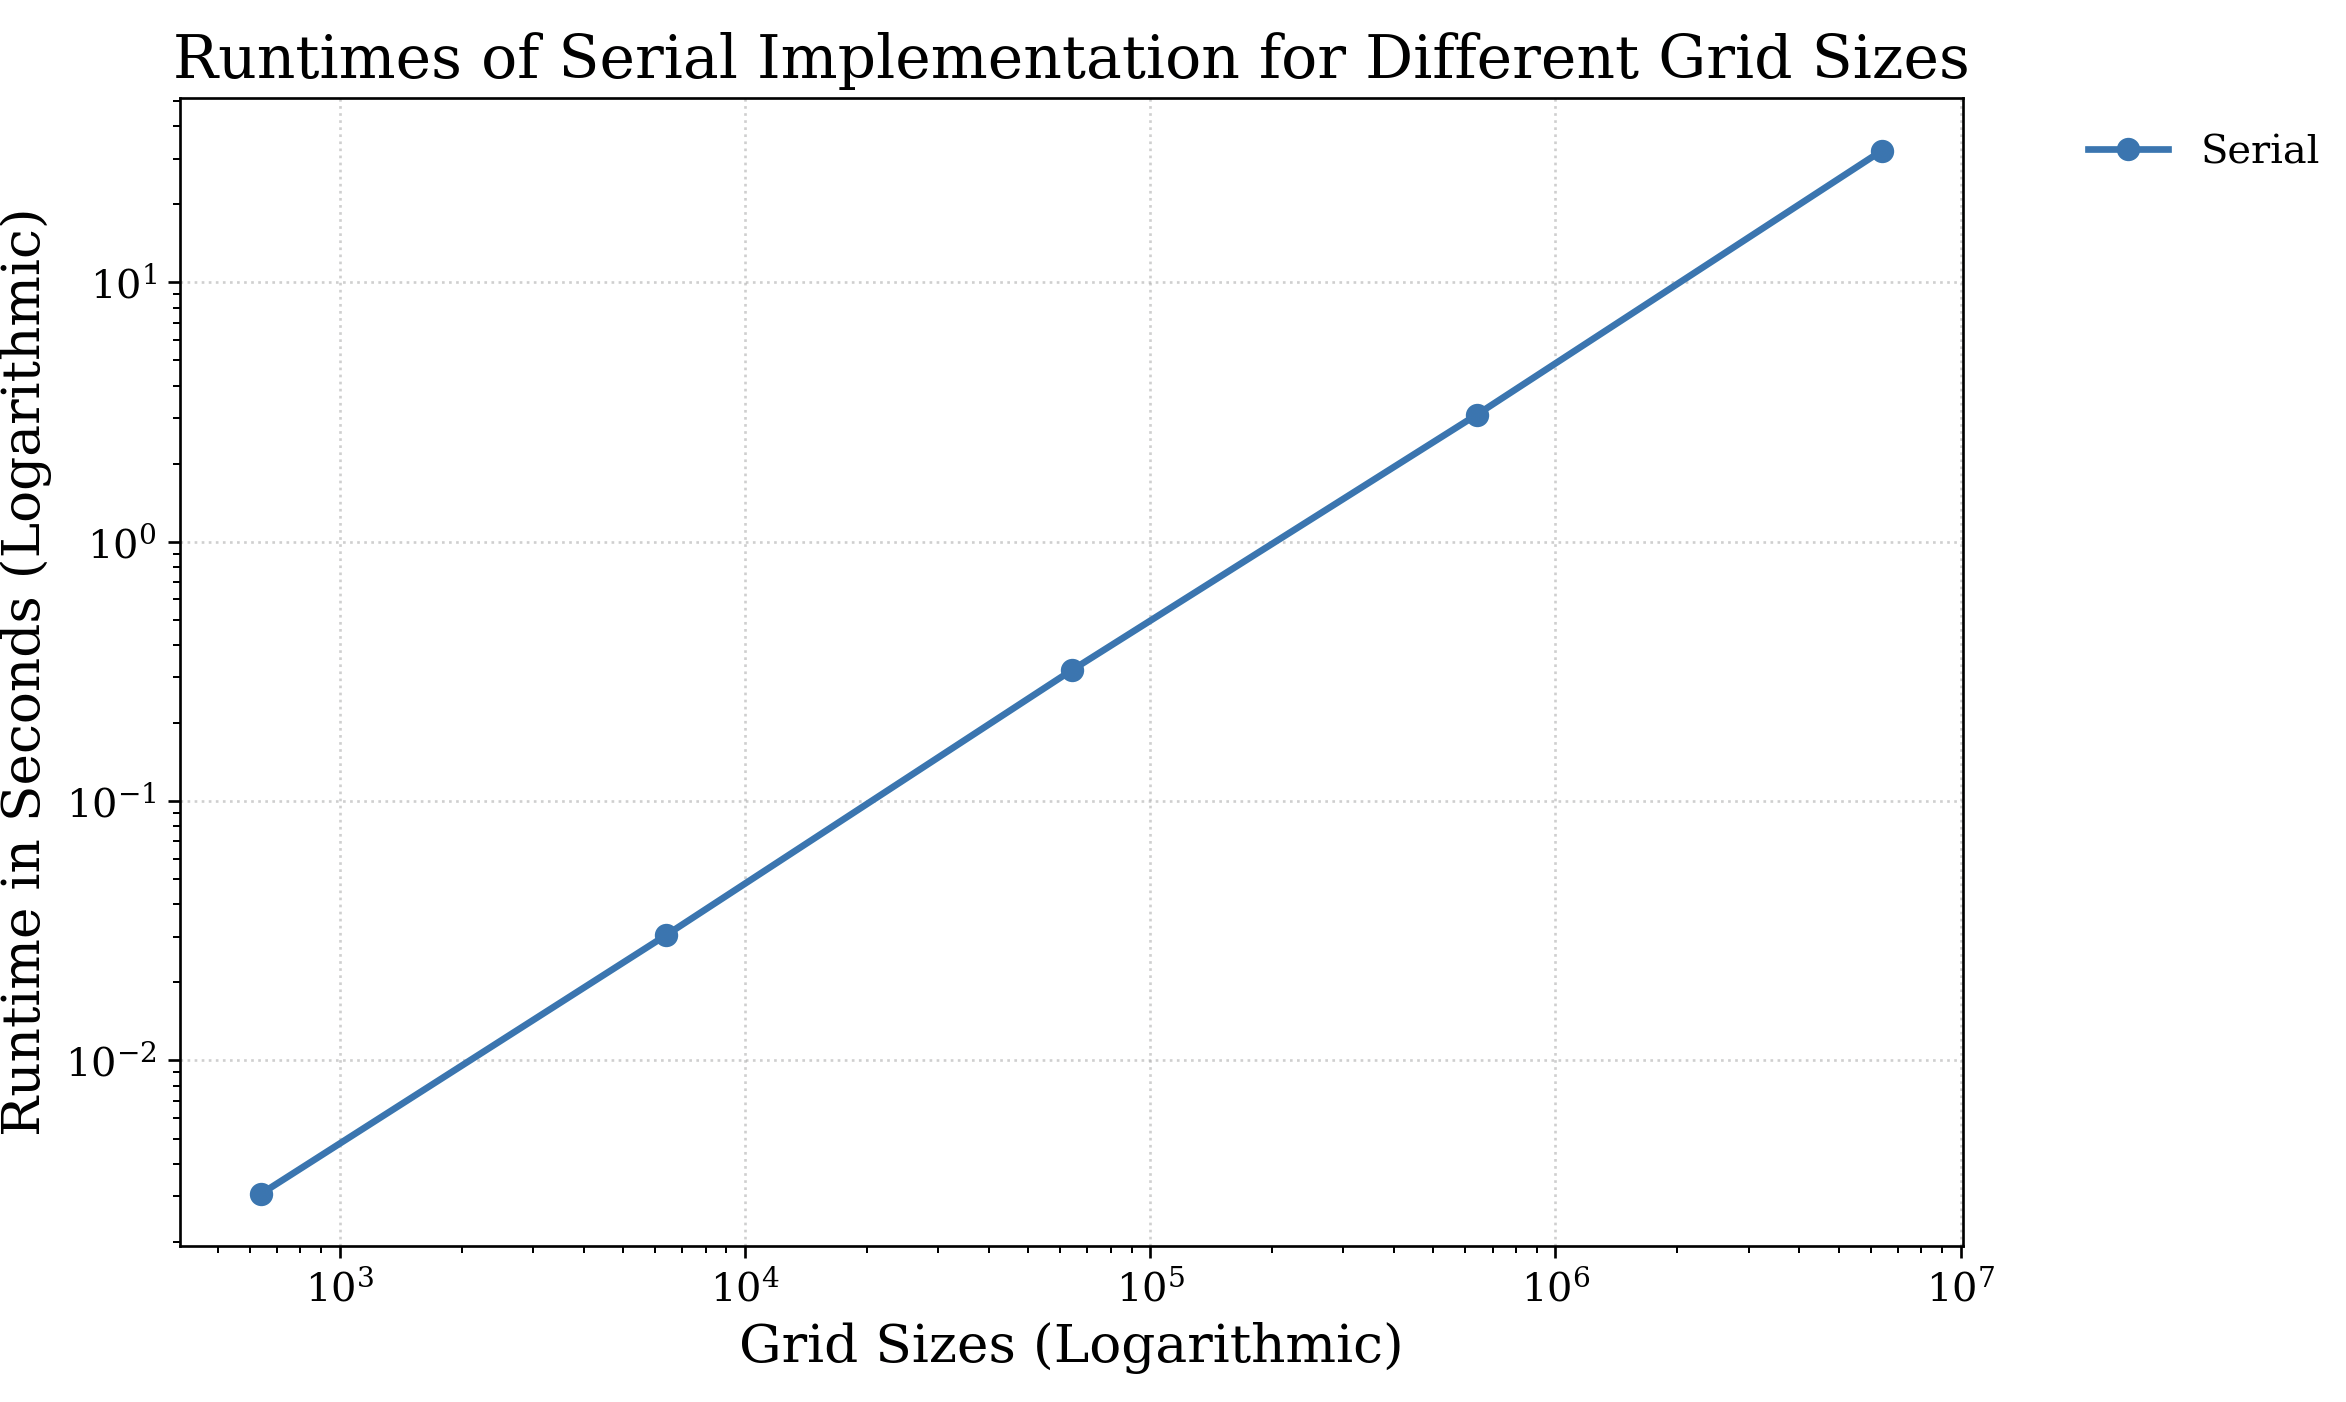
\includegraphics[width=0.9\textwidth]{../images/1_serial/serial_runtime.png}
  \caption{Serial Implementation Runtime}
  \label{fig:1_serial_runtime}
\end{figure}

The results in Figure \ref{fig:1_serial_runtime} are within our expecetations, as we would expect the amount of work to be done (without any parallel intervention) to increase in proportion with the increase in the input size.  

\subsection{Correctness}
We check the implementation correctness of our optimizations against the baseline implementation by visual inspection of the intermediate and final values of the e-field.
To implement this, the e-field values are printed into separate files and matched against each other.
Additionally the peak position at the final time step is validated against the peak position of the serial implementation. 

For both verification methods our results comply with the given code, yielding identical results and showing symmetrical peaks.
\todo{If plots of the final e-field wave are shown, it can be added, that those look like a single Dirac-Impulse instead of two pulses due to scaling, which is shown and proven in the repo. Otherwise this can be removed}

\section{Parallelism through OpenMP}

\section{OpenMP GPU Hand-off}

\section{Parallelism through MPI}
\label{sec:3_mpi}
The code for this section is present in the \verb|3_mpi| directory. The \verb|dardel_runtimes| subdirectory contains the runtimes plotted in the graphs below, which were averages across 3 runs. Additionally, the \verb|outputs/| directory contains the snapshots of \verb|E| and \verb|H| at different time-steps for the serial and parallel implementation(s), which were used to verify correctness using the \verb|verify_outputs.sh| script.

\subsection{Implementation Description}
To parallelize the serial code with the use of MPI, we first initialize the global \verb|E| and \verb|H| grids with the process with rank 0. This is followed by a scattering of this global grid to all processes in the method present \href{https://github.com/paulmyr/DD2356-MethodsHPC/blob/master/5_project/3_mpi/fdtd_mpi.c#L25}{here} in the \verb|fdtd_mpi.c| file. This scattering occurs over a 1D cartesian communicator, which is first created with the help tof \verb|MPI_Cart_create|. 

After this, the following three steps are performed at each step of the update-loop:
\begin{itemize}
\item \underline{Halo-Exchange for E}: Each process sends the first value of the chunk assigned to it to its left neighbour and receives a value in return from its right neighbour. This is done through the blocking \verb|Sendrecv| method to make the exchange easier to reason about. 
\item \underline{Compute H}: The update for the \verb|H| array are performed. These would have required the most up-to-date values for \verb|E|, which is why the halo exchange for \verb|E| occurred in the previous step. We take special care of the boundary condition for \verb|H| when the process performing the update is responsible for the last chunk of \verb|H|.
\item \underline{Halo-Exchange for H}: Each process sends the last value of its updated \verb|H| chunk to its right neighbour and receives a value from its legt neighbour. This is done in an analogous way to the halo-exchange for \verb|E|. 
\item \underline{Compute E}: We finally update the contents of \verb|E|, using the updated values from the \verb|H| ghost cells received in the previous step. This is done in an analogous manner to the updates to \verb|H|, with care taken of the boundary condition in case the process is updating the last chunk of E. 
\end{itemize}

Note that here, all halo-cell exchanges are performed through \underline{blocking, synchronous} communication. Finally, once the computation loop is complete, we add a barrier to ensure that all processes agree to completing all steps of the computation before proceeding. After this barrier, we gather the results of the local \verb|E| and \verb|H| arrays from each process in to a global \verb|E| and \verb|H| grid (respectively) at the rank 0 process in \href{https://github.com/paulmyr/DD2356-MethodsHPC/blob/master/5_project/3_mpi/fdtd_mpi.c#L108}{this} function. This can then be printed to file for diagnostic purposes if needed. The full-code for our implmenetation briefly described above can be found in the \verb|fdtd_mpi.c| file \href{https://github.com/paulmyr/DD2356-MethodsHPC/blob/master/5_project/3_mpi/fdtd_mpi.c}{here}.

\subsection{Strong and Weak Scaling + Communication Overhead}
\label{sec:3_mpi_analysis}

\begin{figure}[H]
     \centering
     \begin{subfigure}[b]{0.45\textwidth}
         \centering
         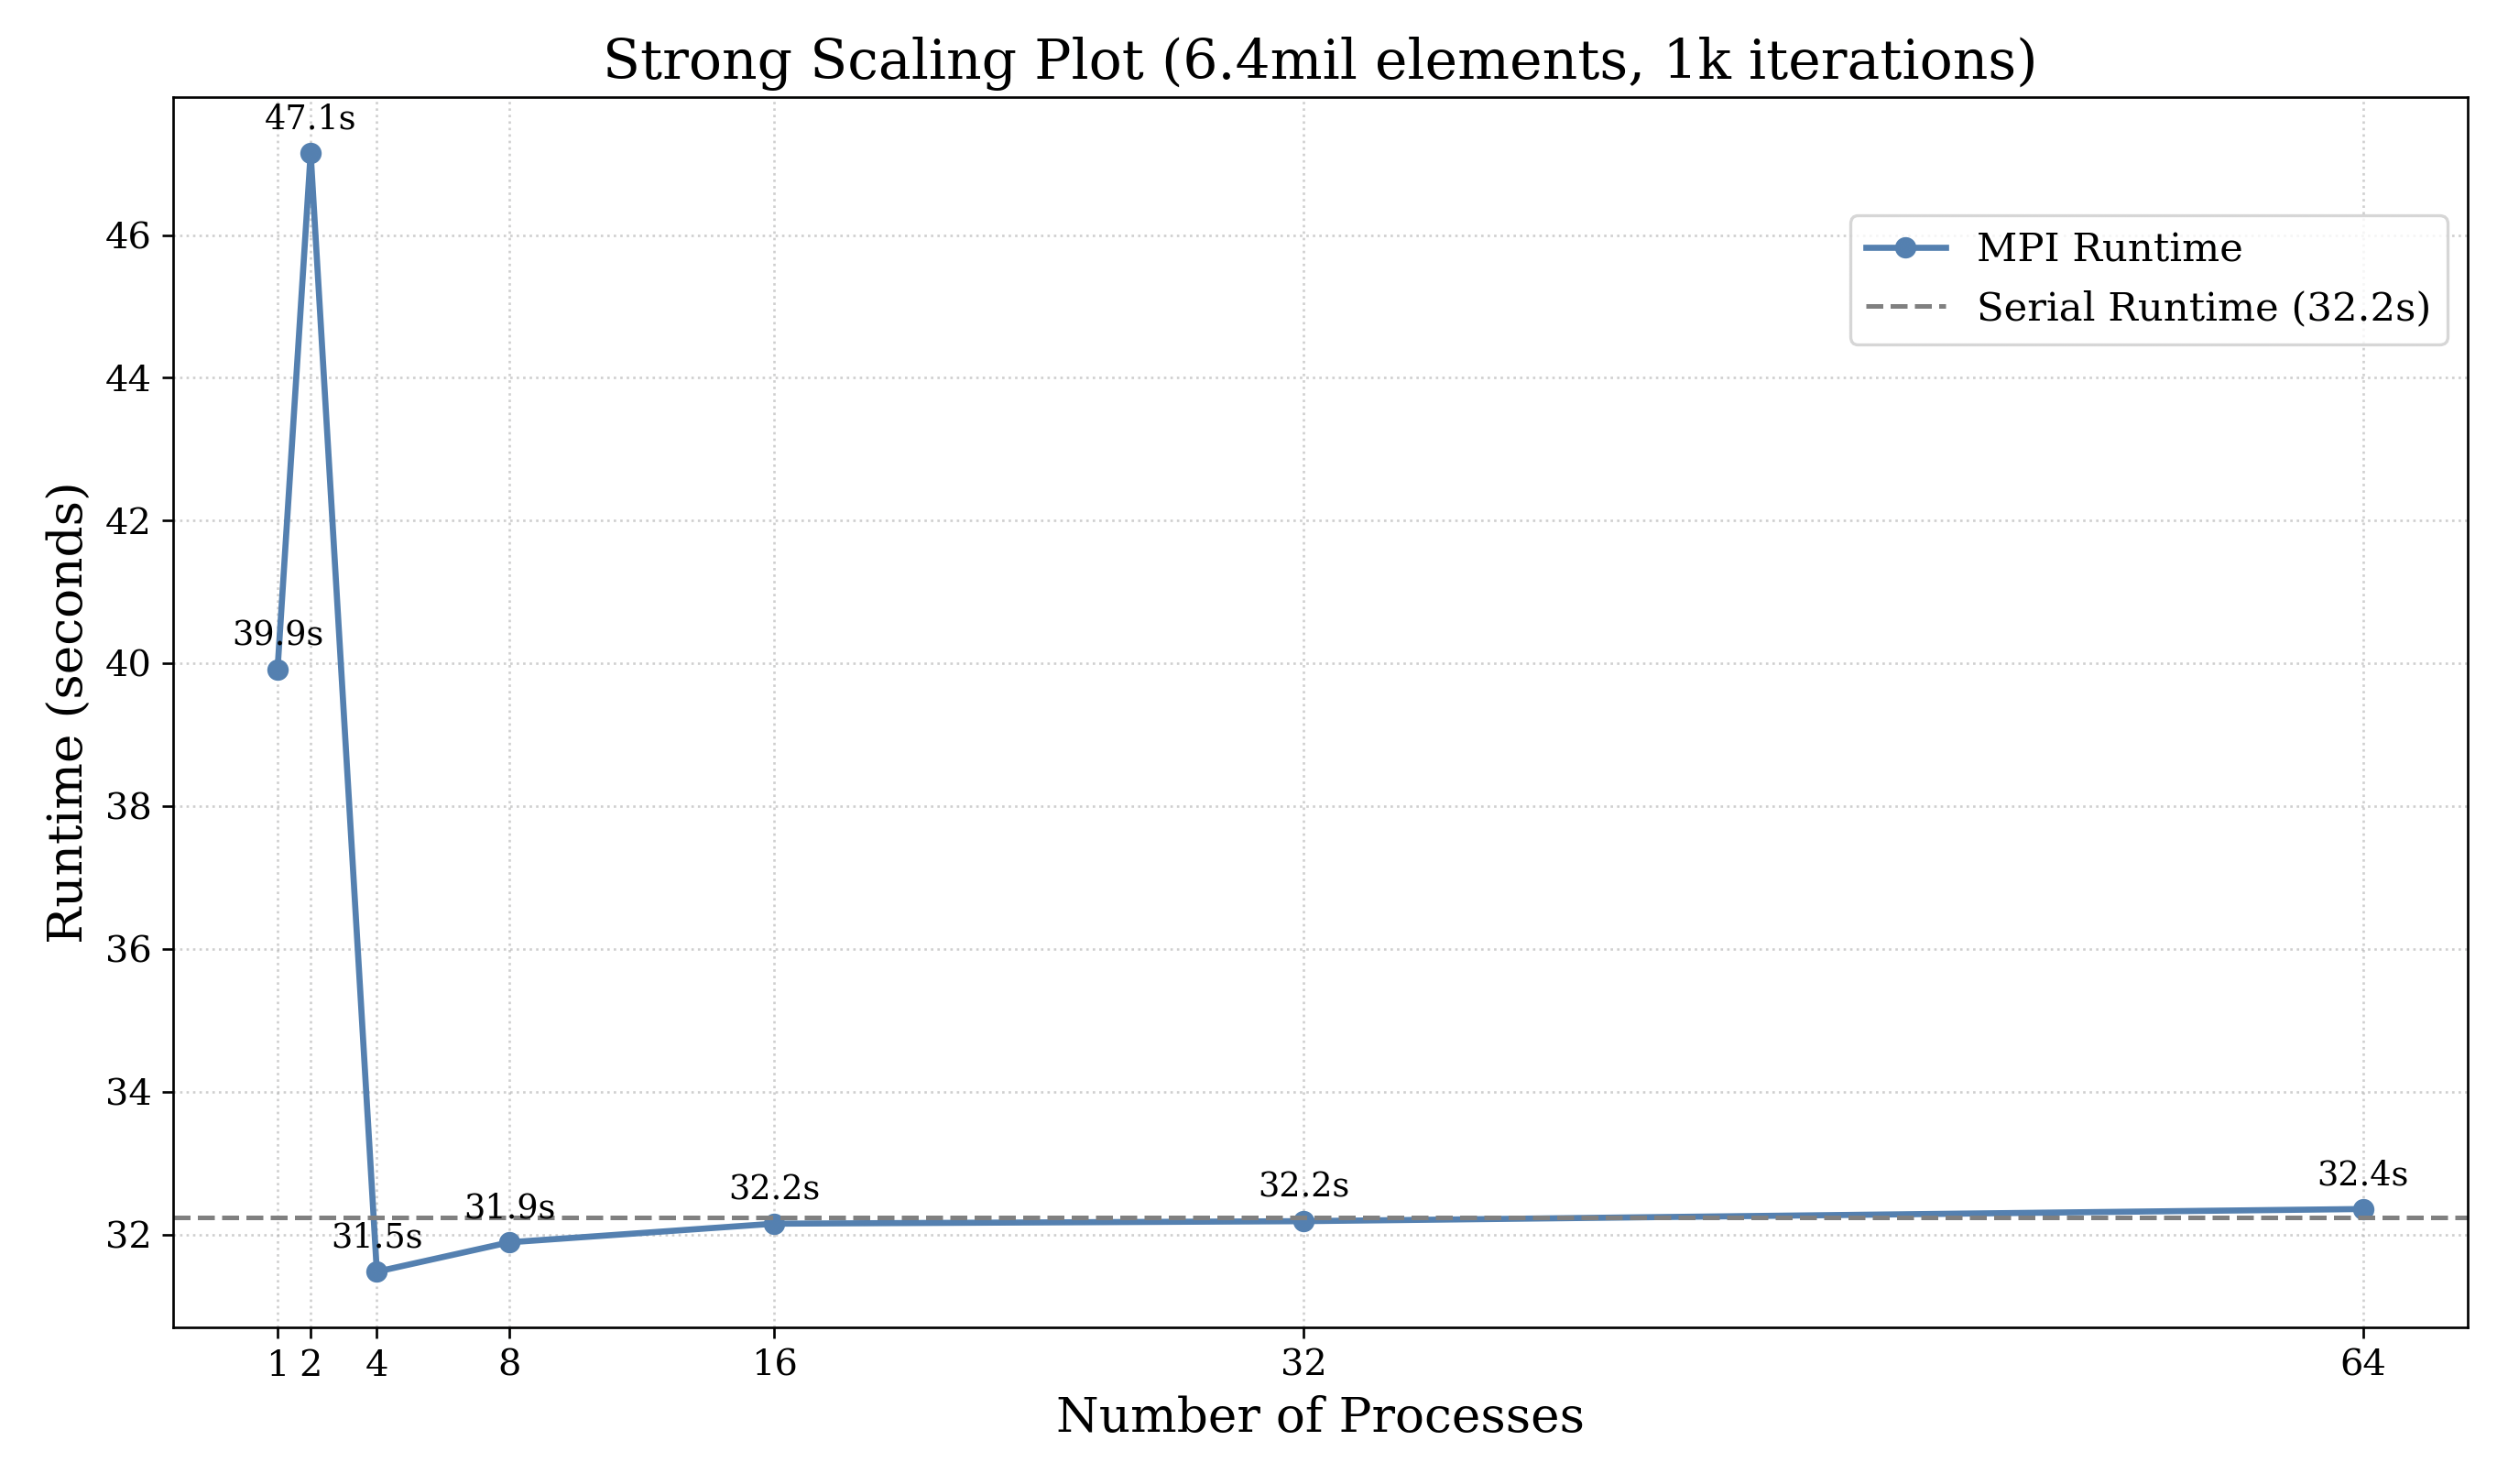
\includegraphics[width=\textwidth]{../images/3_mpi/strong_scaling.png}
         \caption{Strong Scaling (6.4 mil, 1k iters)}
         \label{fig:3_mpi_strong_scaling}
     \end{subfigure}
     \hfill
     \begin{subfigure}[b]{0.45\textwidth}
         \centering
         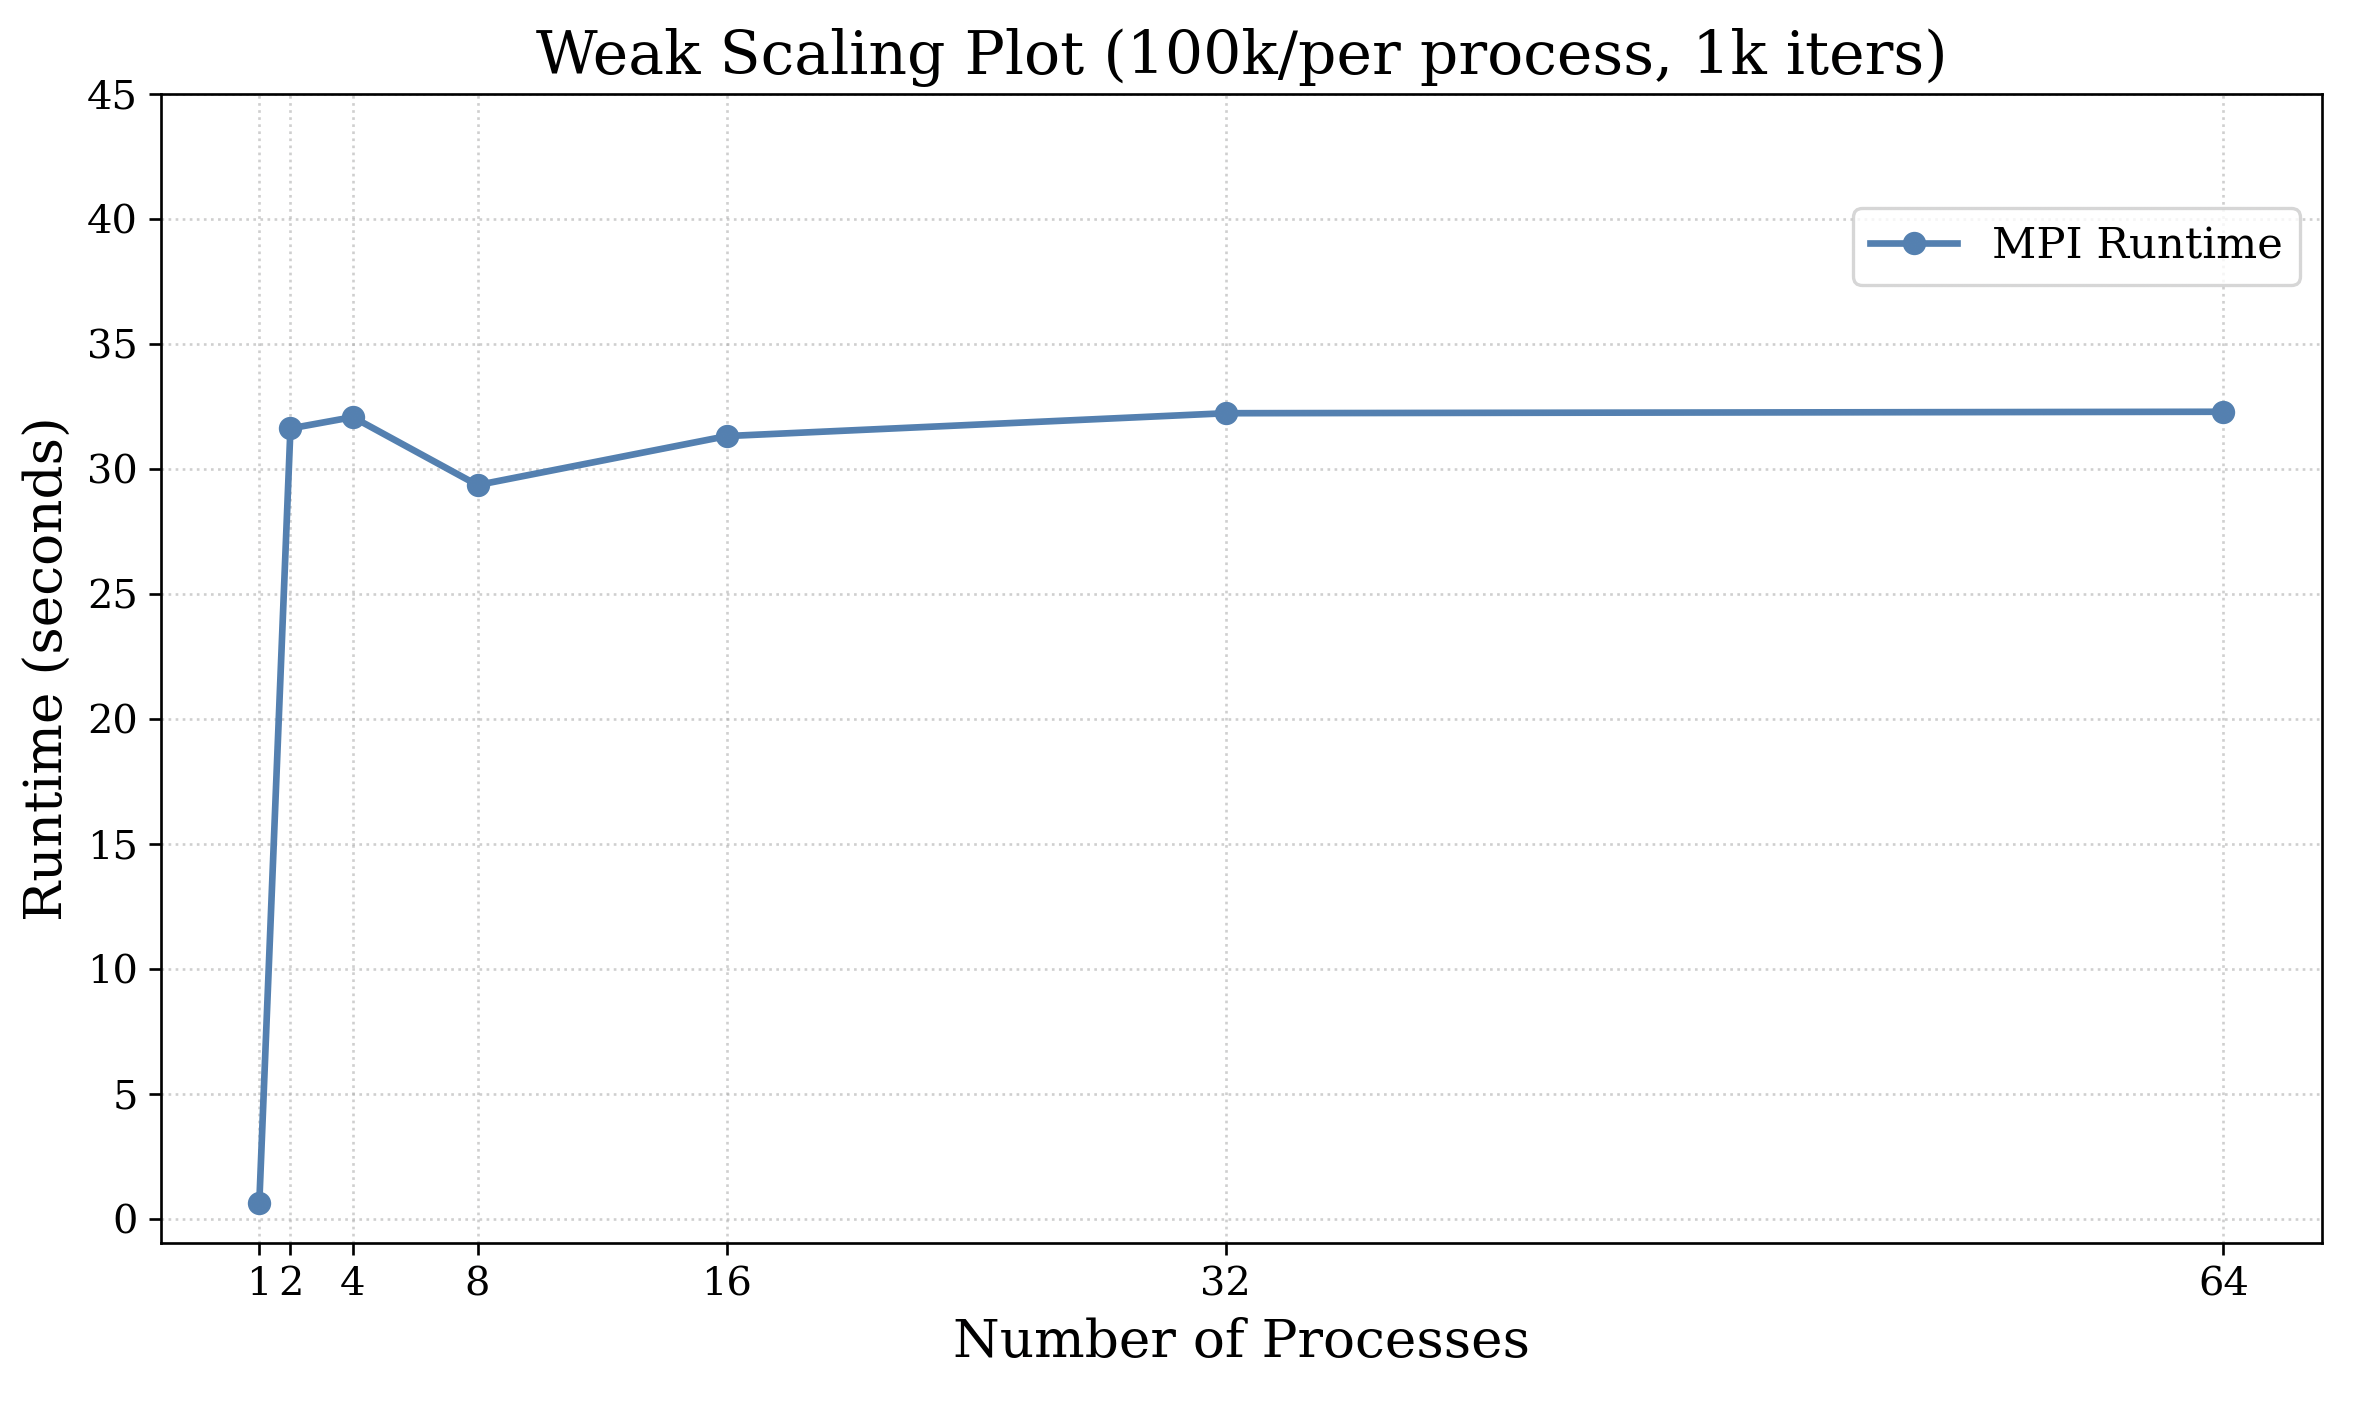
\includegraphics[width=\textwidth]{../images/3_mpi/weak_scaling.png}
         \caption{Weak Scaling (100k/process, 1k iters)}
         \label{fig:3_mpi_weak_scaling}
     \end{subfigure}
     \caption{Strong and Weak Scaling (MPI) }
     \label{fig:3_mpi_strong_weak}
\end{figure}

The strong and weak scaling plot for the implementation can be found in Figure \ref{fig:3_mpi_strong_weak}. The configurations used to generate these runtimes can be found in the \verb|run_strong_scaling.sh| and \verb|run_weak_scaling.sh| files.

From Figure \ref{fig:3_mpi_strong_scaling}, we see worse runtimes for 1 or 2 processes, which could be attributed to the greater MPI overhead compared to the benefits of the limited parallelism through 1 or 2 processes. As the number of processes increase, the runtimes are marginally better -- achieving their lowest at 4 processes and then increasing till they get slightly worse at 64 processes. This trend indicates that the benefits of parallelism start to diminish as the number of processes increase, likely because of greater MPI overhead (halo-exchange, barrier at the end of the compute-loop, etc). Thus, a balance is struck at 4 processes between MPI overhead and parallelism which is optimal. However, there isn't a big variation in the runtimes at $\geq$ 4 processes. Thus, it could be the case that a different run could give better runtimes at 8 processes instead of 4. However, the sharp decline in runtime from 2 to 4 processes shows the promise of MPI parallelism if we use 4-8 processes. 

Figure \ref{fig:3_mpi_weak_scaling} shows that after a sharp increase in runtime going from 1 to 2 processes, the runtime seems to be in the stable 29-33 second range for all process counts. The ideal scenario for a weak-scaling test would be to have runtimes remain stable as the problem size increases -- as this would indicate that larger problems can be solved with the help of larger resources. Except for the jump on going from 1 to 2 processes (because of the MPI overhead with regards to blocking halo-exchanges, etc), we see this ideal trend we hoped for in the weak-scaling test. 

\begin{figure}[H]
  \centering
  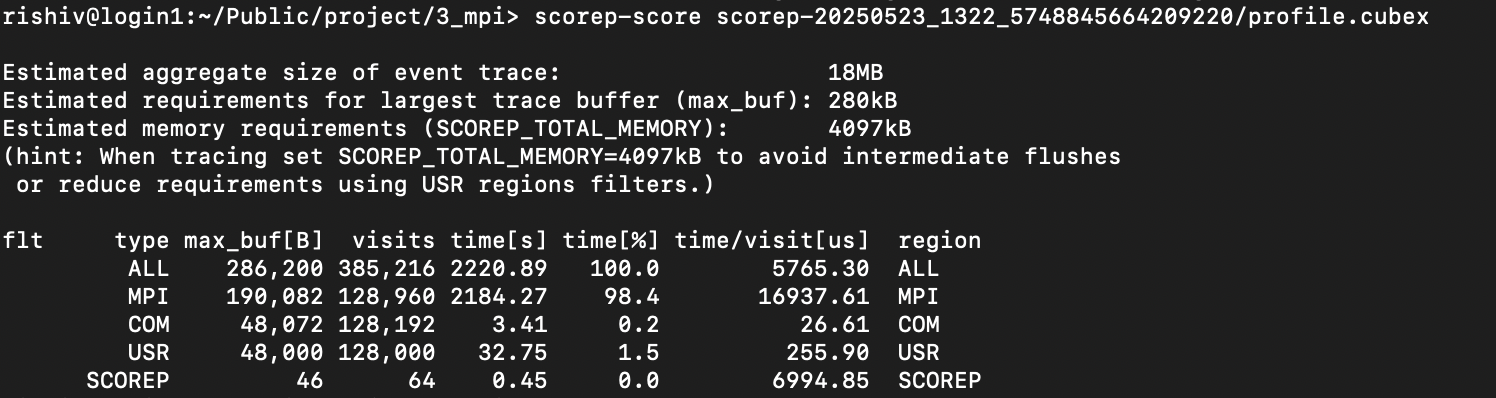
\includegraphics[width=0.9\textwidth]{../images/4_opt/scorep_64_mpi.png}
  \caption{ScoreP on MPI (6.4 Million Elements, 1k Iters, 64 Processes, 1 Node)}
  \label{fig:3_mpi_scorep_64}
\end{figure}

In addition to these tests, we profiled this MPI implementation with ScoreP to get an idea of communication overhead involved with halo-exchanges, using 6.4 million elements and 1k iterations with 64 processes on 1 Node. The results of this can be seen in Figure \ref{fig:3_mpi_scorep_64}. 

We notice a considerably large amount of time being spent in the \verb|MPI| portion of code at a staggering $98.4\%$ of the total time and an incredibly high \verb|time/visit|. The MPI calls done in the compute-loop we are interested in are the blocking \verb|Sendrecv| communication calls for halo-exchanges. Thus, this indicates that because of its blocking nature, each \verb|Sendrecv| call is costing a significant amount of time, bumping up the communication overhead and thus the runtime (total time and time per visit) for the MPI section. In comparison, the \verb|USR| section has a similar number of visits but a drastically lower time spent per visit. This might also explain why we did not see a significant improvement in runtime compared to the serial version as the number of processes increase -- any benefit gained from parallelism was likely countered by the overhead of blocking communication between more processes. With an increase in the number of processes, the subproblem size and the chunk of the compute loop gets smaller. Hence, more time is spent waiting for halo-exchanges to complete than in the local computation by each process. Thus, performing halo exchanges in a non-blocking manner could lead to some improvements, which is what guided our optimization strategy in the next section.

\section{Optimizing MPI Parallelism}
For optimization of the parallel implementations, we focus on the parallel MPI implementation in Section \ref{sec:3_mpi}. The OpenMP implementations were incredibly fast compared to the serial counterparts already, and we felt we could improve MPI a lot more. The files referred to in this section can be found under the \verb|4_opt| directory of the repository. The \verb|dardel_runtimes/| and the \verb|outputs/| directory serve the same purpose as in Section \ref{sec:3_mpi}.

\subsection{Attempt 1: Communication-Computation Overlap w/ Non-Blocking Halo Exchange}
\label{sec:async_mpi}
From the ScoreP analysis of the MPI code in Section \ref{sec:3_mpi_analysis}, we concluded that the blocking \verb|Sendrecv| halo-exchanges are likely contributing to the lackluster performance. To rectify this issue, we decided to implement halo-exchanges through non-blocking mechanisms: with the help of \verb|Irecv| and \verb|Isend|. This allowed us to overlap communiation (through halo-exchanges) with computation: since the \textit{interior} portion of each chunk can be computed without the need of data from halo-exchanges.

Thus, we initiate  \verb|Irecv| and \verb|Isend| requests for a halo-exchange, then compute the updated values for the interior of each chunk. After this computation, we \textit{wait} on these 2 halo-exchange requests to complete, after which we compute the boundary cell(s). We repeat this method for updating both the \verb|E| and the \verb|H| grids. The code for this can be found in the \verb|fdtd_async_opt.c|. We will refer to this as the \underline{Async/Non-Blocking Optimization (Opt 1)} of the MPI code from Section \ref{sec:3_mpi}, while the code from Section \ref{sec:3_mpi} will be referred to as the \underline{Base MPI} implementation.

Figure \ref{fig:4_opt1} shows the performance of this optimization compared to the blocking/base MPI implementation from Section \ref{sec:3_mpi}. We vary the number of processes keeping the problem size constant (6.4 million elements, 1k iterations). The script for obtaining these runtimes can be found in the \verb|run_async_opt.sh| file \href{https://github.com/paulmyr/DD2356-MethodsHPC/blob/master/5_project/4_opt/run_async_opt.sh}{here}. From Figure \ref{fig:4_opt1}, we can see that till 8 processes, the async MPI imeplementation performs visibly better than the synchronous version. We believe that the reason for this is the communication-computation overlap to update the interior of the grids makes more efficient use of the idle time that was otherwise wasted in the synchronous halo-exchange.

However, the performance from 16 processes onwards is quite similar, where any differences between the two runs could likely be attributed to being within a margin of error from each other. Thus, this shows that with an increase in the number of processes, the cost of synchronizing the MPI communication between different/adjacent workers adds up -- negating the potential benefits of the asynchronous exchange. Additonally, as the number of processes increase but the problem size remains the same, we have more processes responsible for smaller chunks of the global arrays. This means that the \textit{computation} part of the computation-communication overlap is smaller, and thus the processes are more likely to end up waiting for a longer time at the \verb|MPI_Waitall| call after the interior-computation is finished. This would give us similar behaviour to the sync MPI implementation, which is what we observed.


\begin{figure}[H]
     \centering
     \begin{subfigure}[b]{0.45\textwidth}
         \centering
         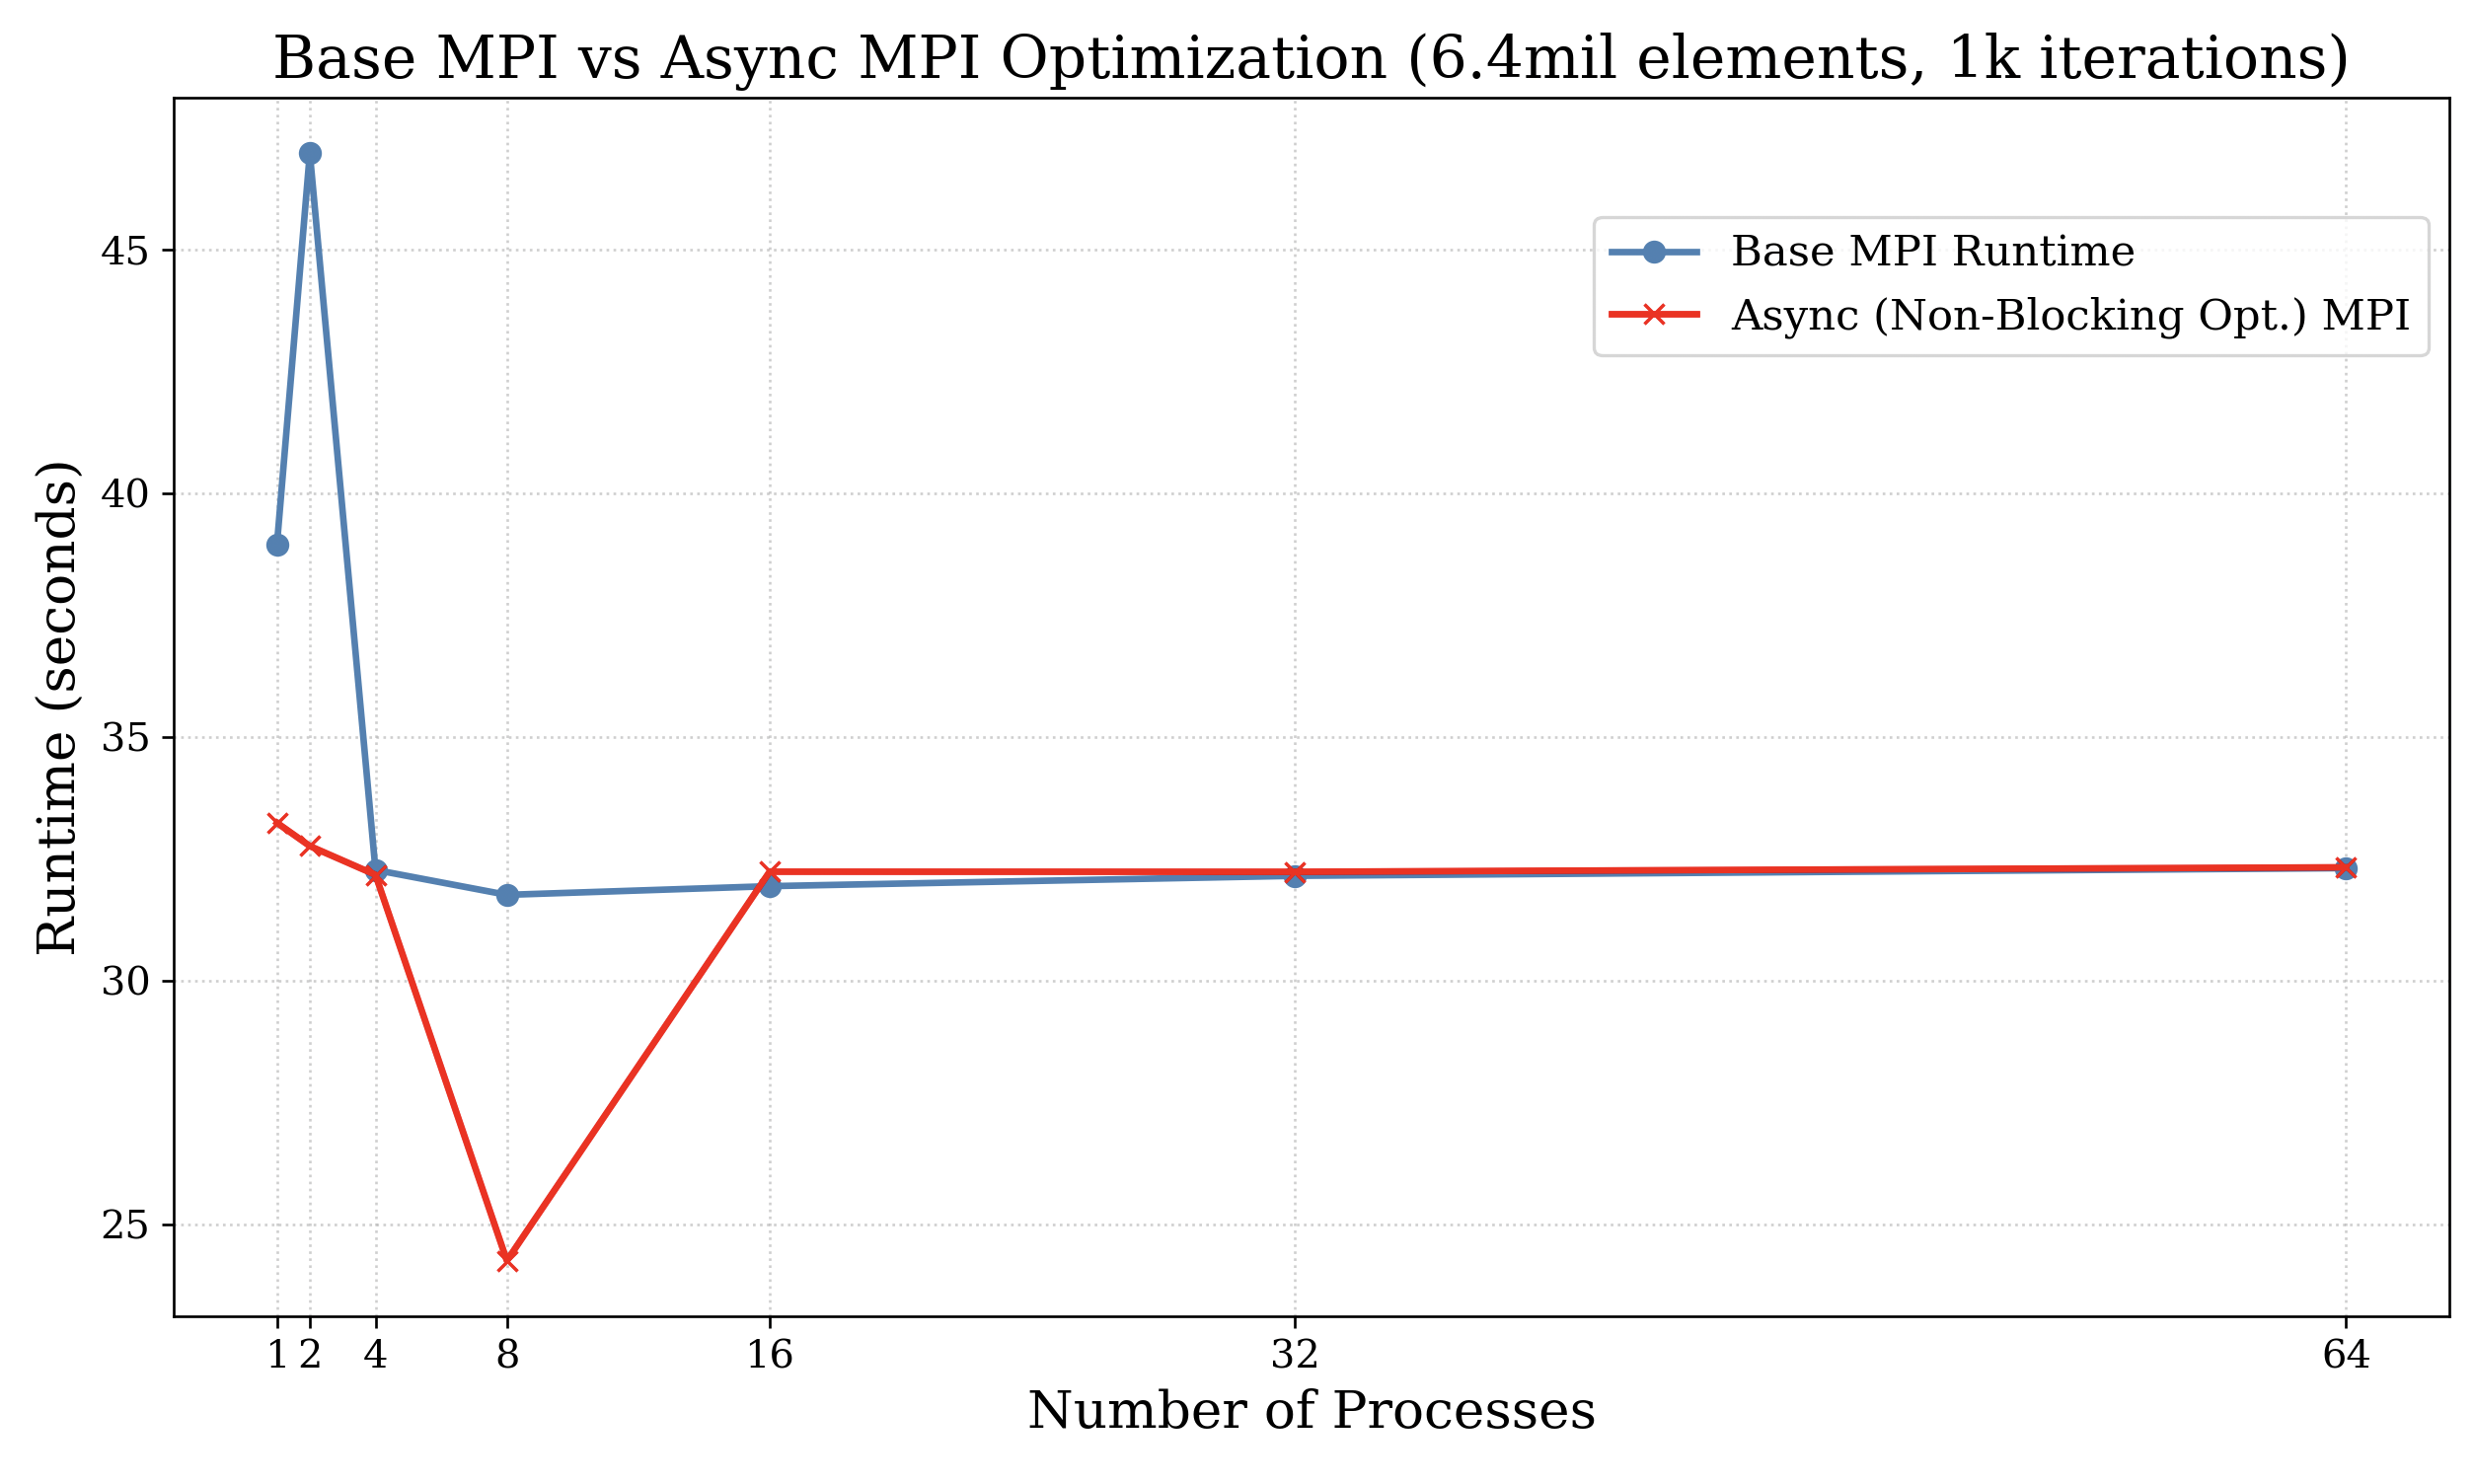
\includegraphics[width=\textwidth]{../images/4_opt/opt1.png}
         \caption{Varying Processes (Same Input)}
         \label{fig:4_opt1}
     \end{subfigure}
     \hfill
     \begin{subfigure}[b]{0.45\textwidth}
         \centering
         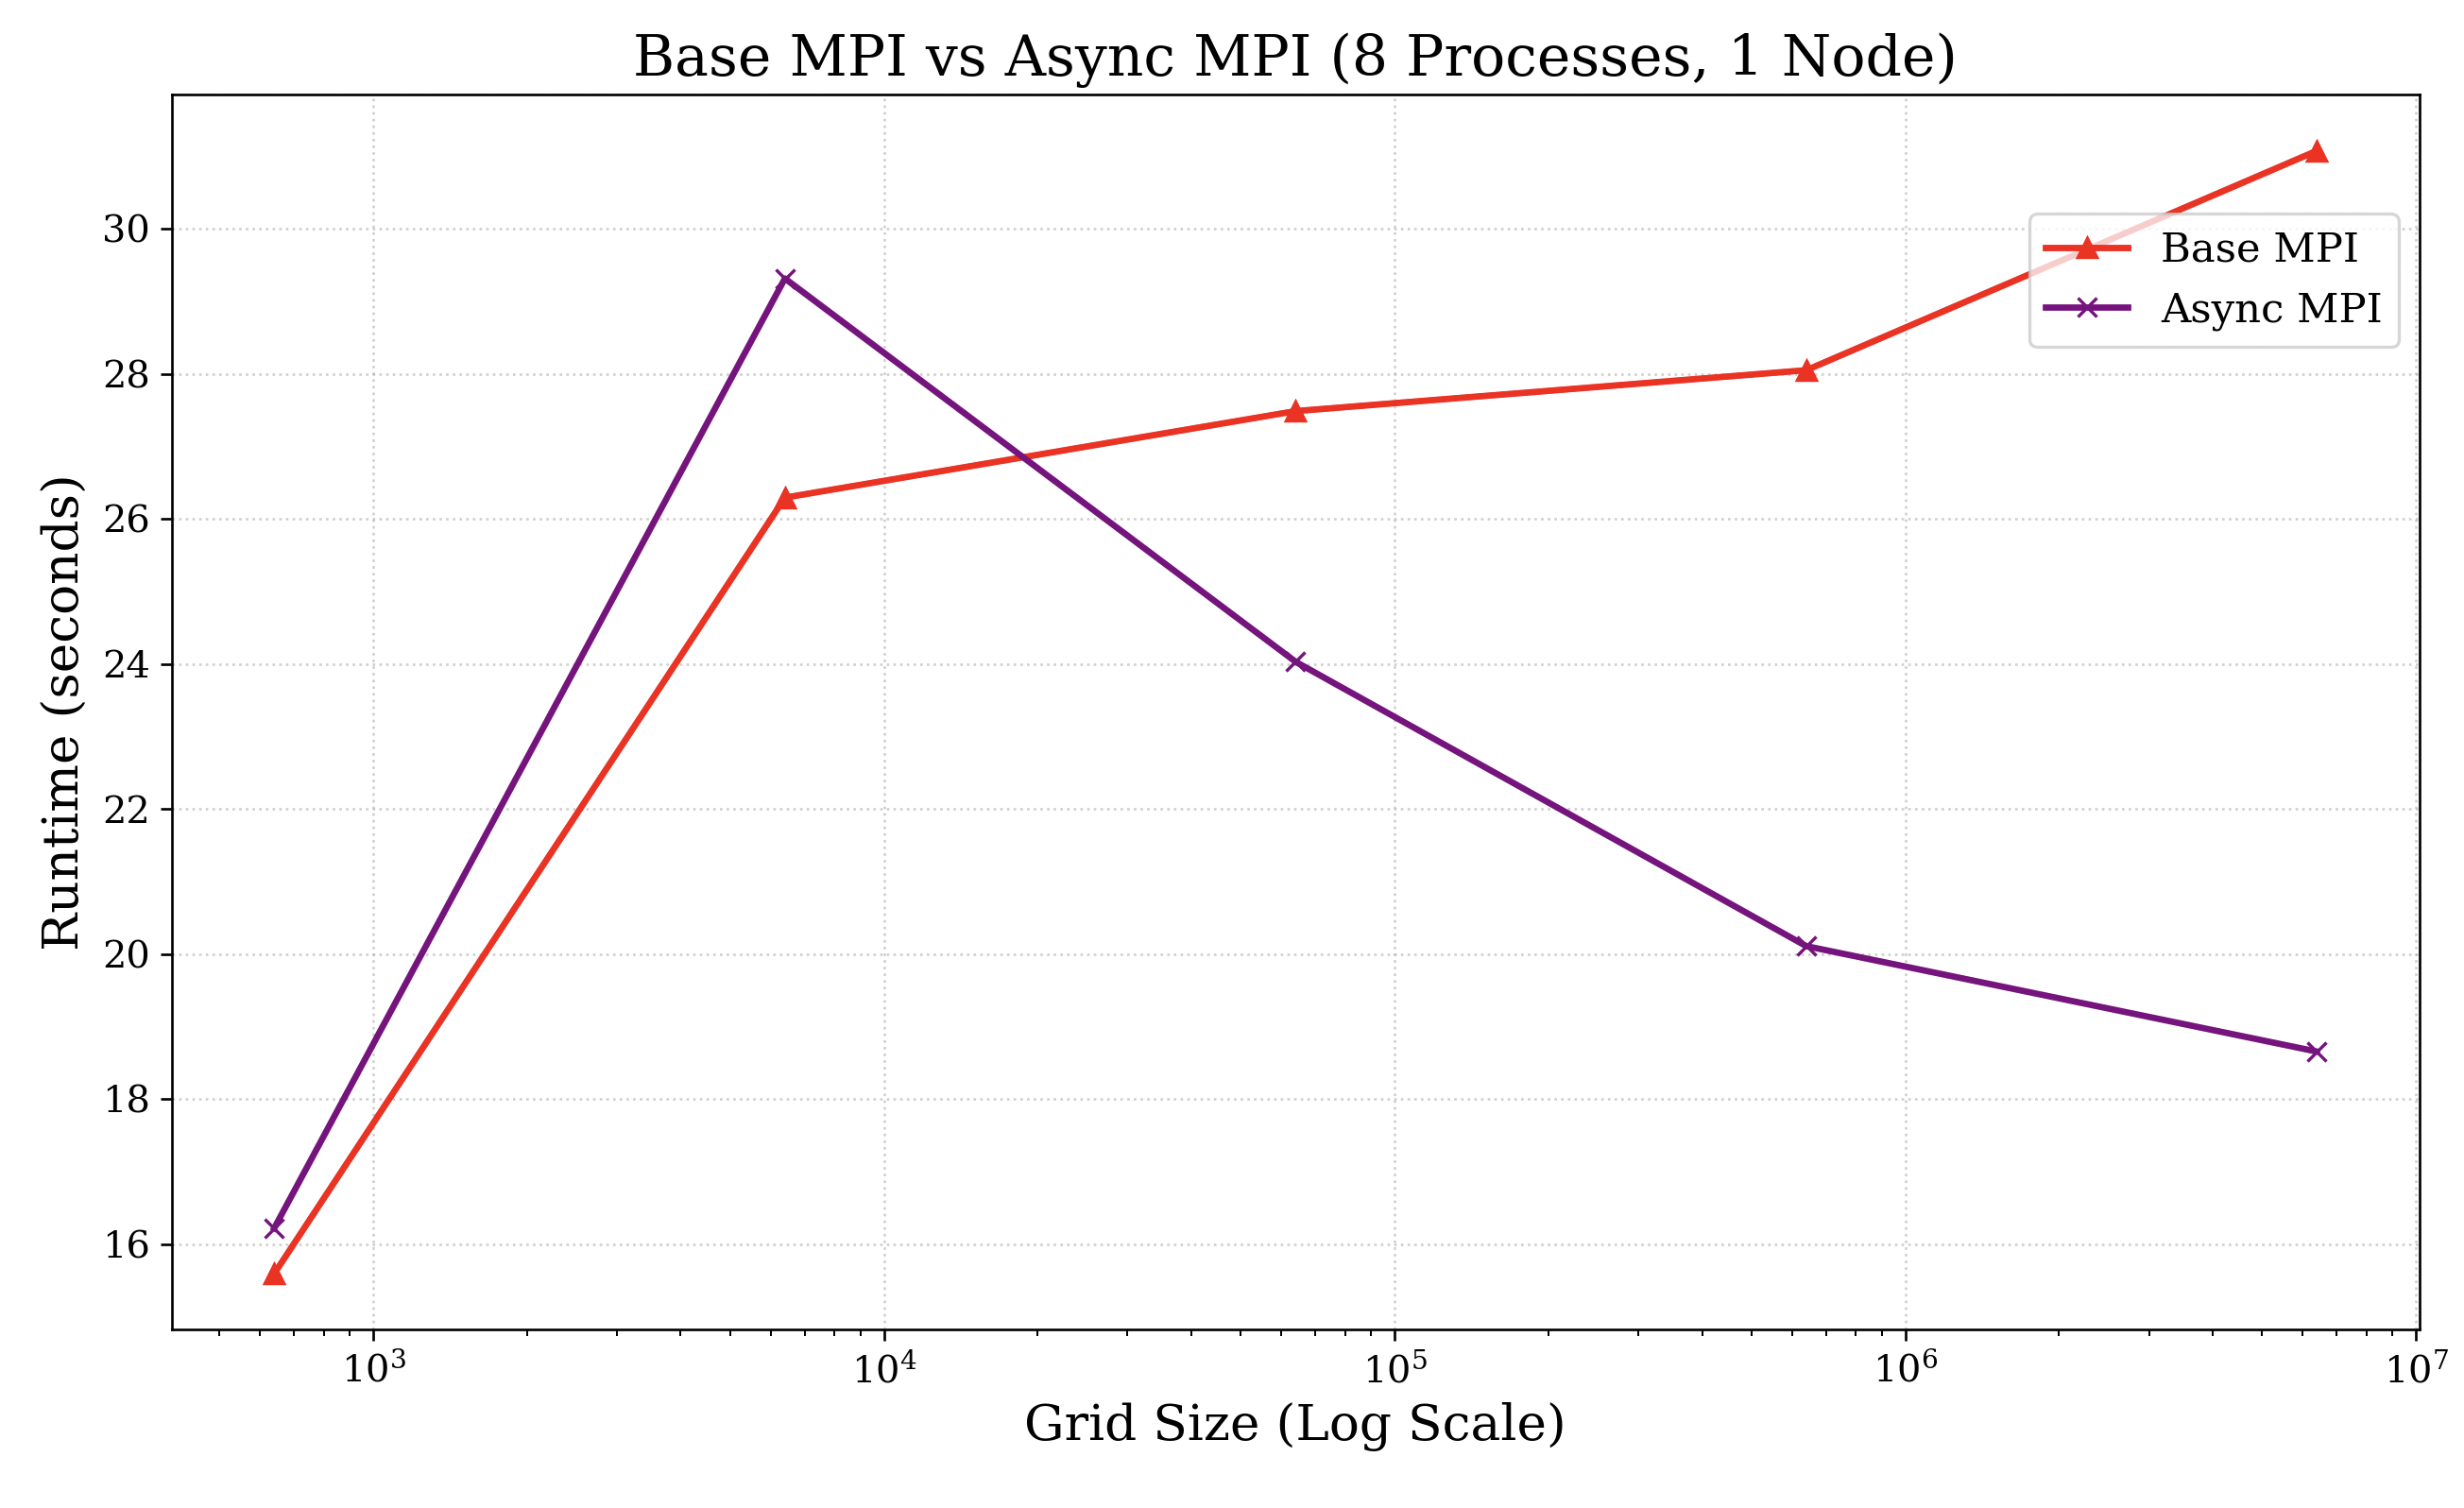
\includegraphics[width=\textwidth]{../images/4_opt/opt_compare_8.png}
         \caption{Varying Input (8 Processes)}
         \label{fig:4_opt_compare_8}
     \end{subfigure}
     \caption{Sync (Base) MPI vs Async MPI}
     \label{fig:4_opt_async_runtimes}
\end{figure}

Based on the results from Figure \ref{fig:4_opt1}, we concluded that 8 processes seems to offer the best balance between async MPI communication and parallelism, and wanted to explore this further. This was done in Figure \ref{fig:4_opt_compare_8}, where we analyzed the runtimes across different grid sizes for the 2 implementations, both using 8 processes. The SLURM script for this can be found in the \verb|run_mpi_async_opt_compare.sh| file \href{https://github.com/paulmyr/DD2356-MethodsHPC/blob/master/5_project/4_opt/run_mpi_async_opt_compare.sh}{here}. For smaller grid sizes, the two implementations seem to perform similarly, with the Base MPI even having a slight edge likely because of the simpler structure of the code and fewer calls to the MPI library making the async communication an unnecessary excess. Another reason might be the smaller \textit{computation} portion because of smaller grid-sizes, as explained earlier.


However, as the grid sizes increase, we start seeing the noticable benefit of using async over sync communication for halo-exchanges. As the grid sizes increase, so does the "computation" part of the overlap, meaning that more time is spent efficiently performing interior-updates before hitting the eventual blocking \verb|MPI_Waitall| call. This call then finishes quickly and brings forth the anticipated advantage.
\textit{Note: While the runtimes plotted in Figure \ref{fig:4_opt_compare_8} are averages across 3 runs, we did observe considerable differences between these runs for both the Base MPI and the Async MPI implementations. We believed this might be because of unexpected allocation of processes to CPUs on the Numa nodes by SLURM (making for variable communication time), and thus requested more processes on the same node to get better allocation. Despite this, we did observe some non-trivial variation between runs on the same invocation. However, the trend we observed seemed to largely follow the one presented here.}


We also profiled using ScoreP the Base MPI and the Async MPI imeplementation using 8 processes (6.4 million elements, 1k iterations). Figure \ref{fig:4_opt_scorep_sync} and Figure \ref{fig:4_opt_scorep_async} show the result of the analysis for the Sync and Async implementations with this configuration, respectively.  
\begin{figure}[H]
     \centering
     \begin{subfigure}[b]{0.45\textwidth}
         \centering
         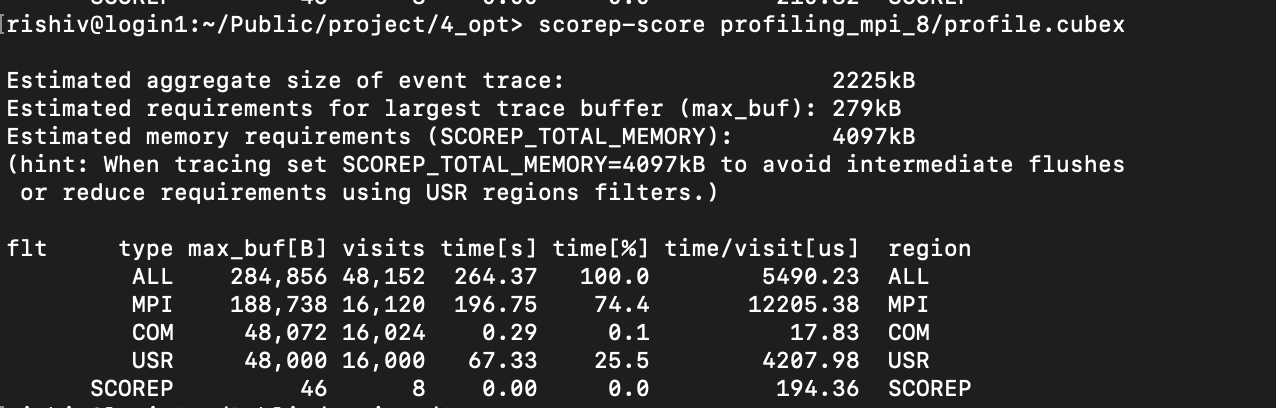
\includegraphics[width=\textwidth]{../images/4_opt/scorep_8_mpi.png}
         \caption{Synchronous (Base) MPI ScoreP}
         \label{fig:4_opt_scorep_sync}
     \end{subfigure}
     \hfill
     \begin{subfigure}[b]{0.45\textwidth}
         \centering
         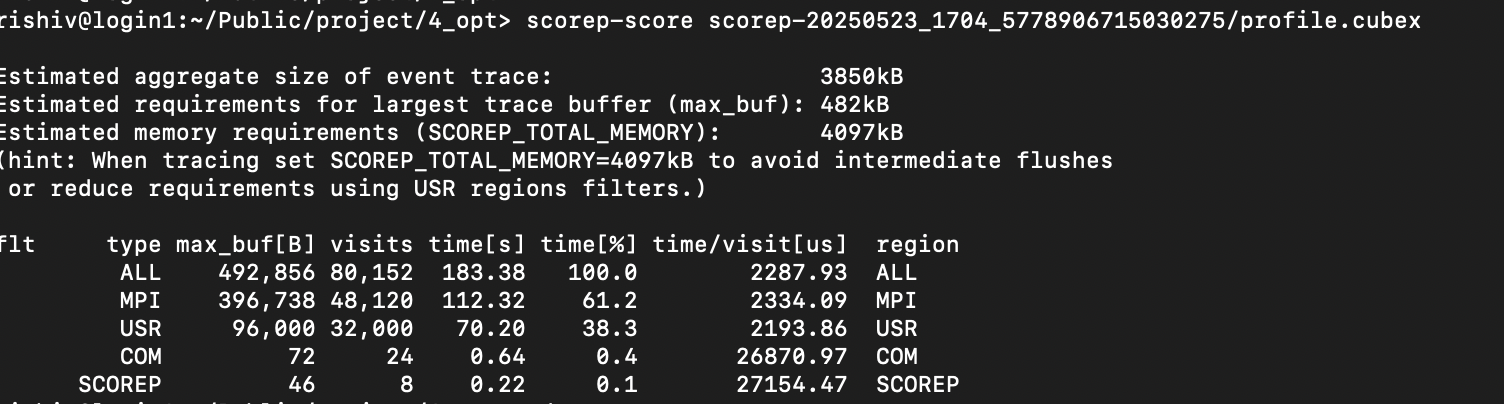
\includegraphics[width=\textwidth]{../images/4_opt/scorep_8_async.png}
         \caption{Async (Optimized) MPI ScoreP}
         \label{fig:4_opt_scorep_async}
     \end{subfigure}
     \caption{Sync (Base) MPI vs Async MPI ScoreP}
\end{figure}

Despite a greater percentage of time being spent in the MPI section for the Async implementation and a higher number of visits to MPI, we notice that the time per call for MPI is significantly lower compared to that for the Sync Implementation. We believe that this is because of the fewer amount of waiting time required near blocking calls (such as \verb|MPI_Waitall|), since the relatively larger computation portion gives enough time for the halo-exchanges to have finished by the time we reach the blocking portion of the code. This is also evident in the total time (for \verb|ALL|) spent in the simulation -- where we see a nearly 30 second decrease in the Async version compared to the Sync version. While the actual running times are likely much higher for both implementations here because of hte ScoreP profiling intervention, a 30 second difference is considerably large, which would likely translate to a noticeable difference \textit{without} ScoreP as well -- as was observed in the plots in Figure \ref{fig:4_opt_async_runtimes}.

\subsection{Attempt 2: OpenMP Parallelism w/ Non-Blocking Halo Exchange}
We investigated if we could obtain noticeable runtime improvements over what was seen in Section \ref{sec:async_mpi}, and were able to do so by incorporating OpenMP into the \verb|E| and \verb|H| updates. The code for this can be found in the \verb|fdtd_async_omp_opt.c| \href{https://github.com/paulmyr/DD2356-MethodsHPC/blob/master/5_project/4_opt/fdtd_async_omp_opt.c}{here}. The main changes here involved the use OpenMP parallelism in the compute-intensive loop-based updates into the \textit{interior} of the chunk that each process is assigned. \href{https://github.com/paulmyr/DD2356-MethodsHPC/blob/master/5_project/4_opt/fdtd_async_omp_opt.c#L61}{This} snippet illustrates this for the \verb|H|-interior updates. 

\todo{Possibly some explanation on why we're using the architecture that we do?}
Given this code, we investigated the impact of spreading the computation on up-to 4 Dardel Nodes , where we spawn up-to 4 processes (meaning we tested on upto 16 processes in total) on each Node and have 16 threads per process. The Slurm file used to obtain the runtimes with this configuration can be found \href{https://github.com/paulmyr/DD2356-MethodsHPC/blob/master/5_project/4_opt/run_async_omp_opt.sh}{here}. 

\begin{figure}[H]
  \centering
  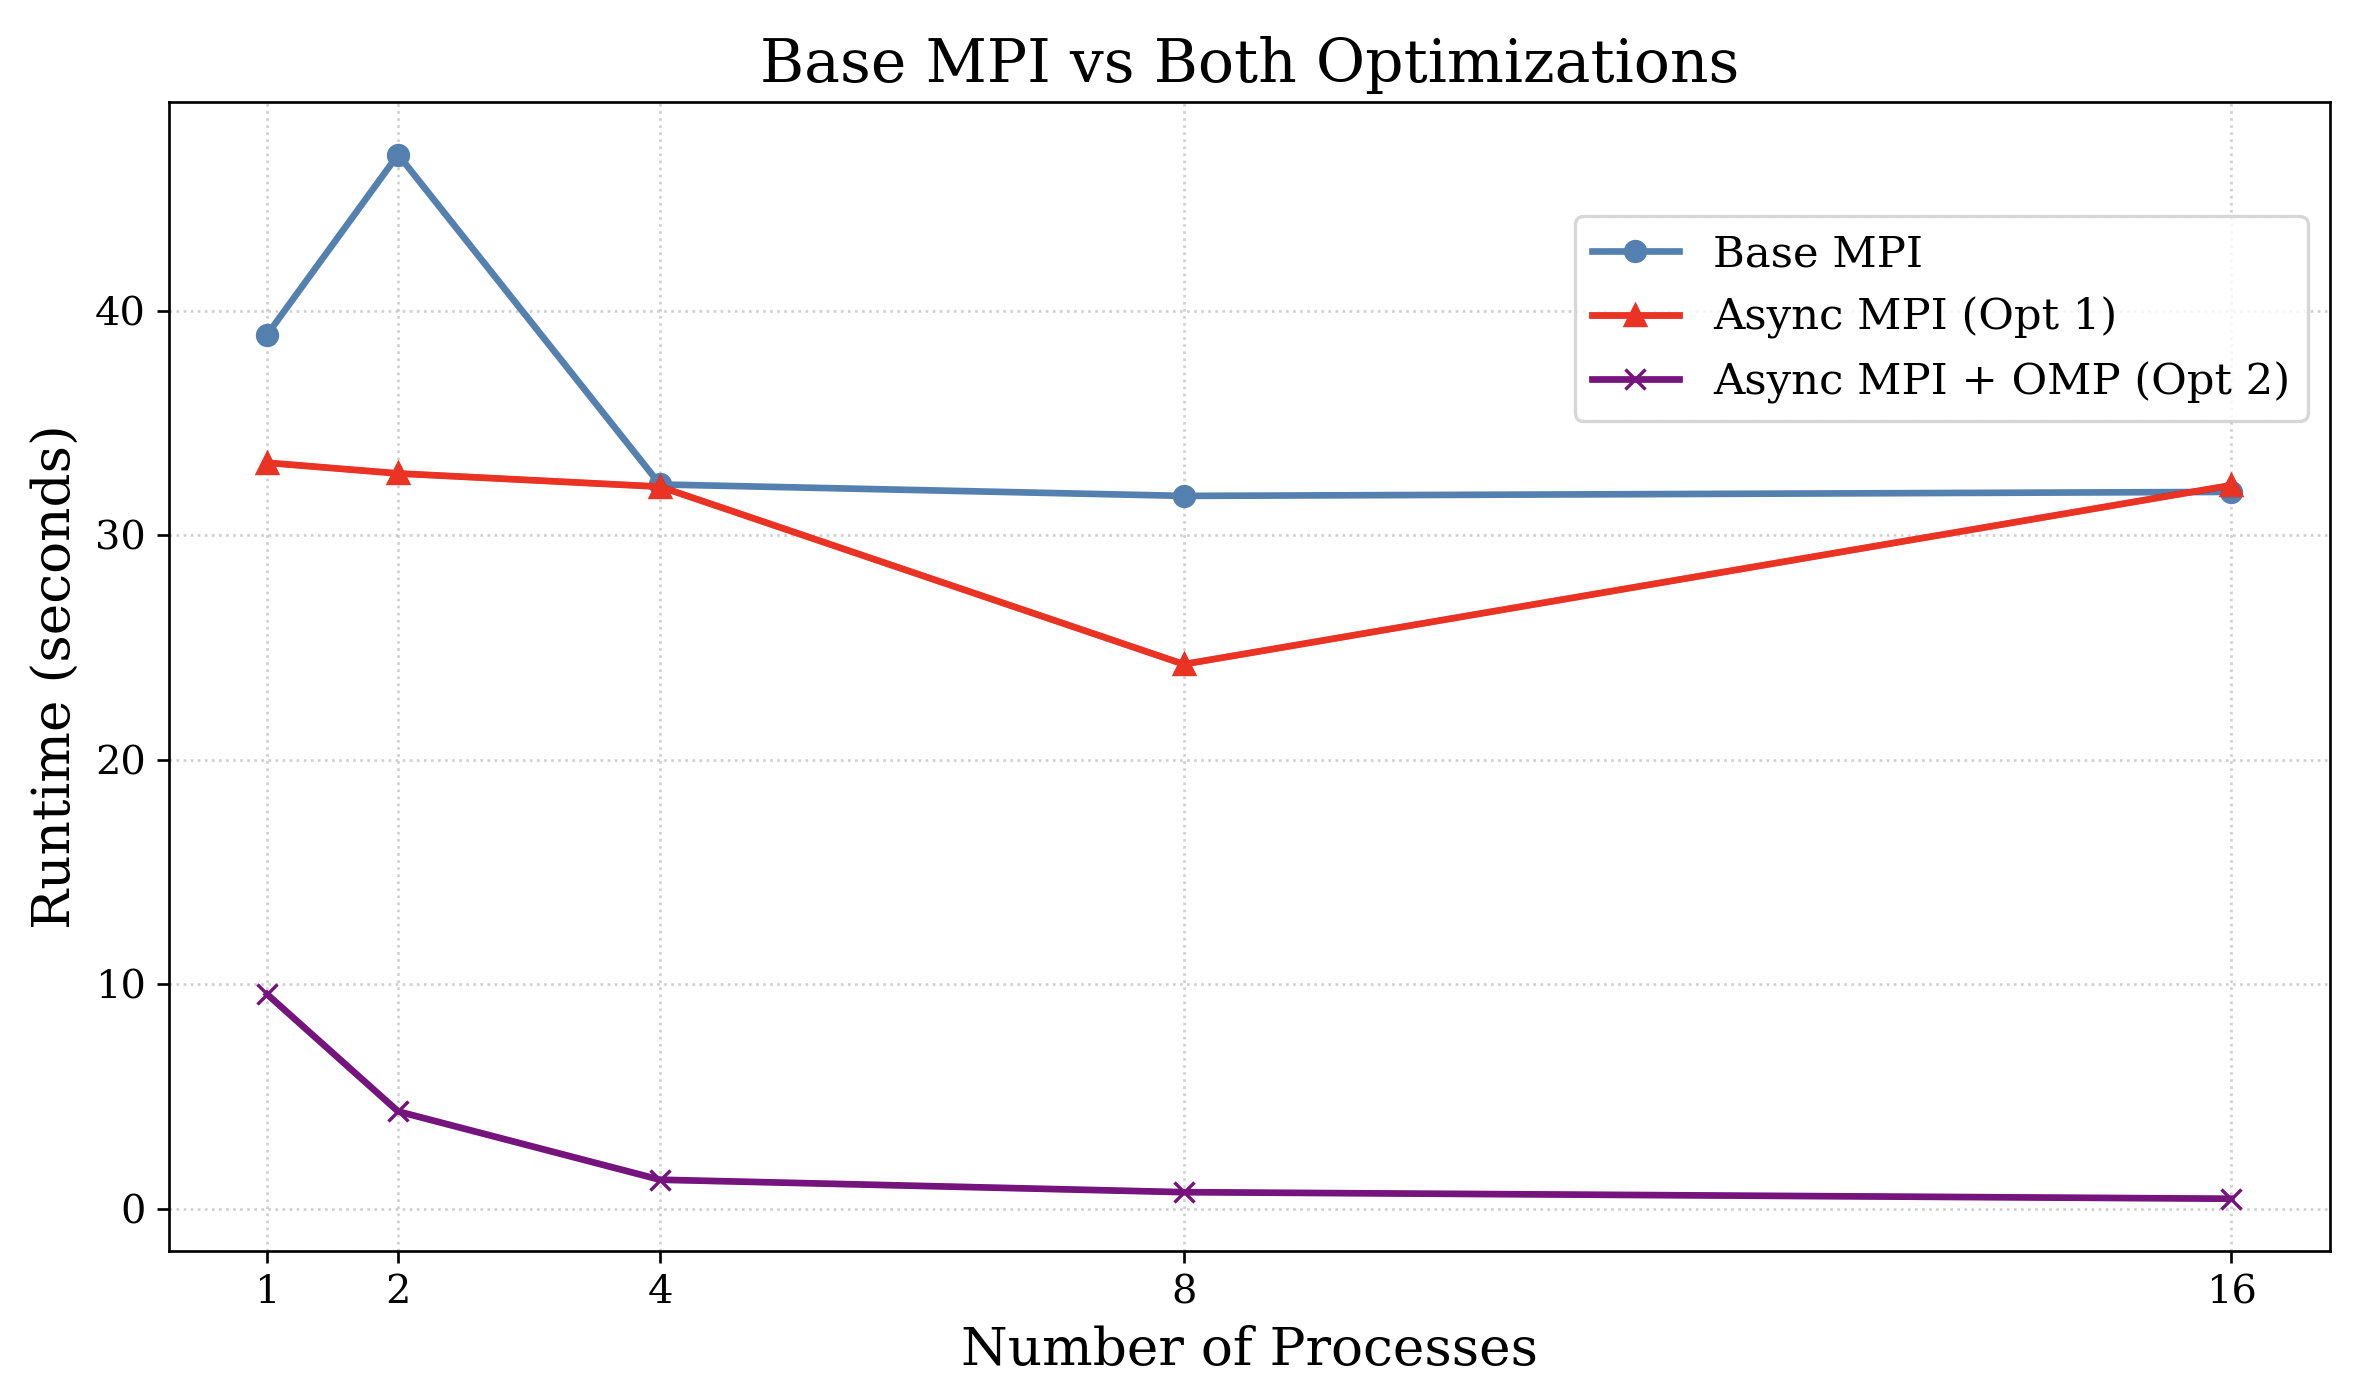
\includegraphics[width=0.9\textwidth]{../images/4_opt/opt_all.png}
  \caption{Async MPI + OMP Performance}
   \label{fig:4_opt_all}
\end{figure}

\todo{Does this explanation make sense?}
Figure \ref{fig:4_opt_all} shows the comparison between the Async MPI + OpenMP implementation with the other two MPI implementations discussed earlier. The problem size is kept constant here (6.4 million elements, 1k iterations). We can see that unlike the Async-only MPI implementation (Optimization 1), the performance of the Async MPI + OpenMP implementation (Optimization 2) continues to improve as we go from 8 processes to 16 processes. One explanation for this could be that the use of OpenMP threads in the compute portion of the communication-compute overlap drastically accelerates the overall runtime of \textit{each step} in the overall simulation. Thus, despite the compute part becoming faster (because of the use of OpenMP) and consequently there being less of an \textit{overlap} between the compute and the communication, Optimization 2 makes each step of the compute more efficient, thus consistently reducing the runtime.

\section{Conclusion}
In the previous sections, we discussed the runtimes of the different implementations and optimizations of the 1D FDTD simulation. Here, we present a final graph with the runtimes of each of the implementations discussed plotted against the serial runtime as we increase the grid size. For implementations that can have different configurations (such as: different number of threads in OpenMP), we have plotted the runtimes of the best configuration observed while examining the section. 

\begin{figure}[H]
  \centering
  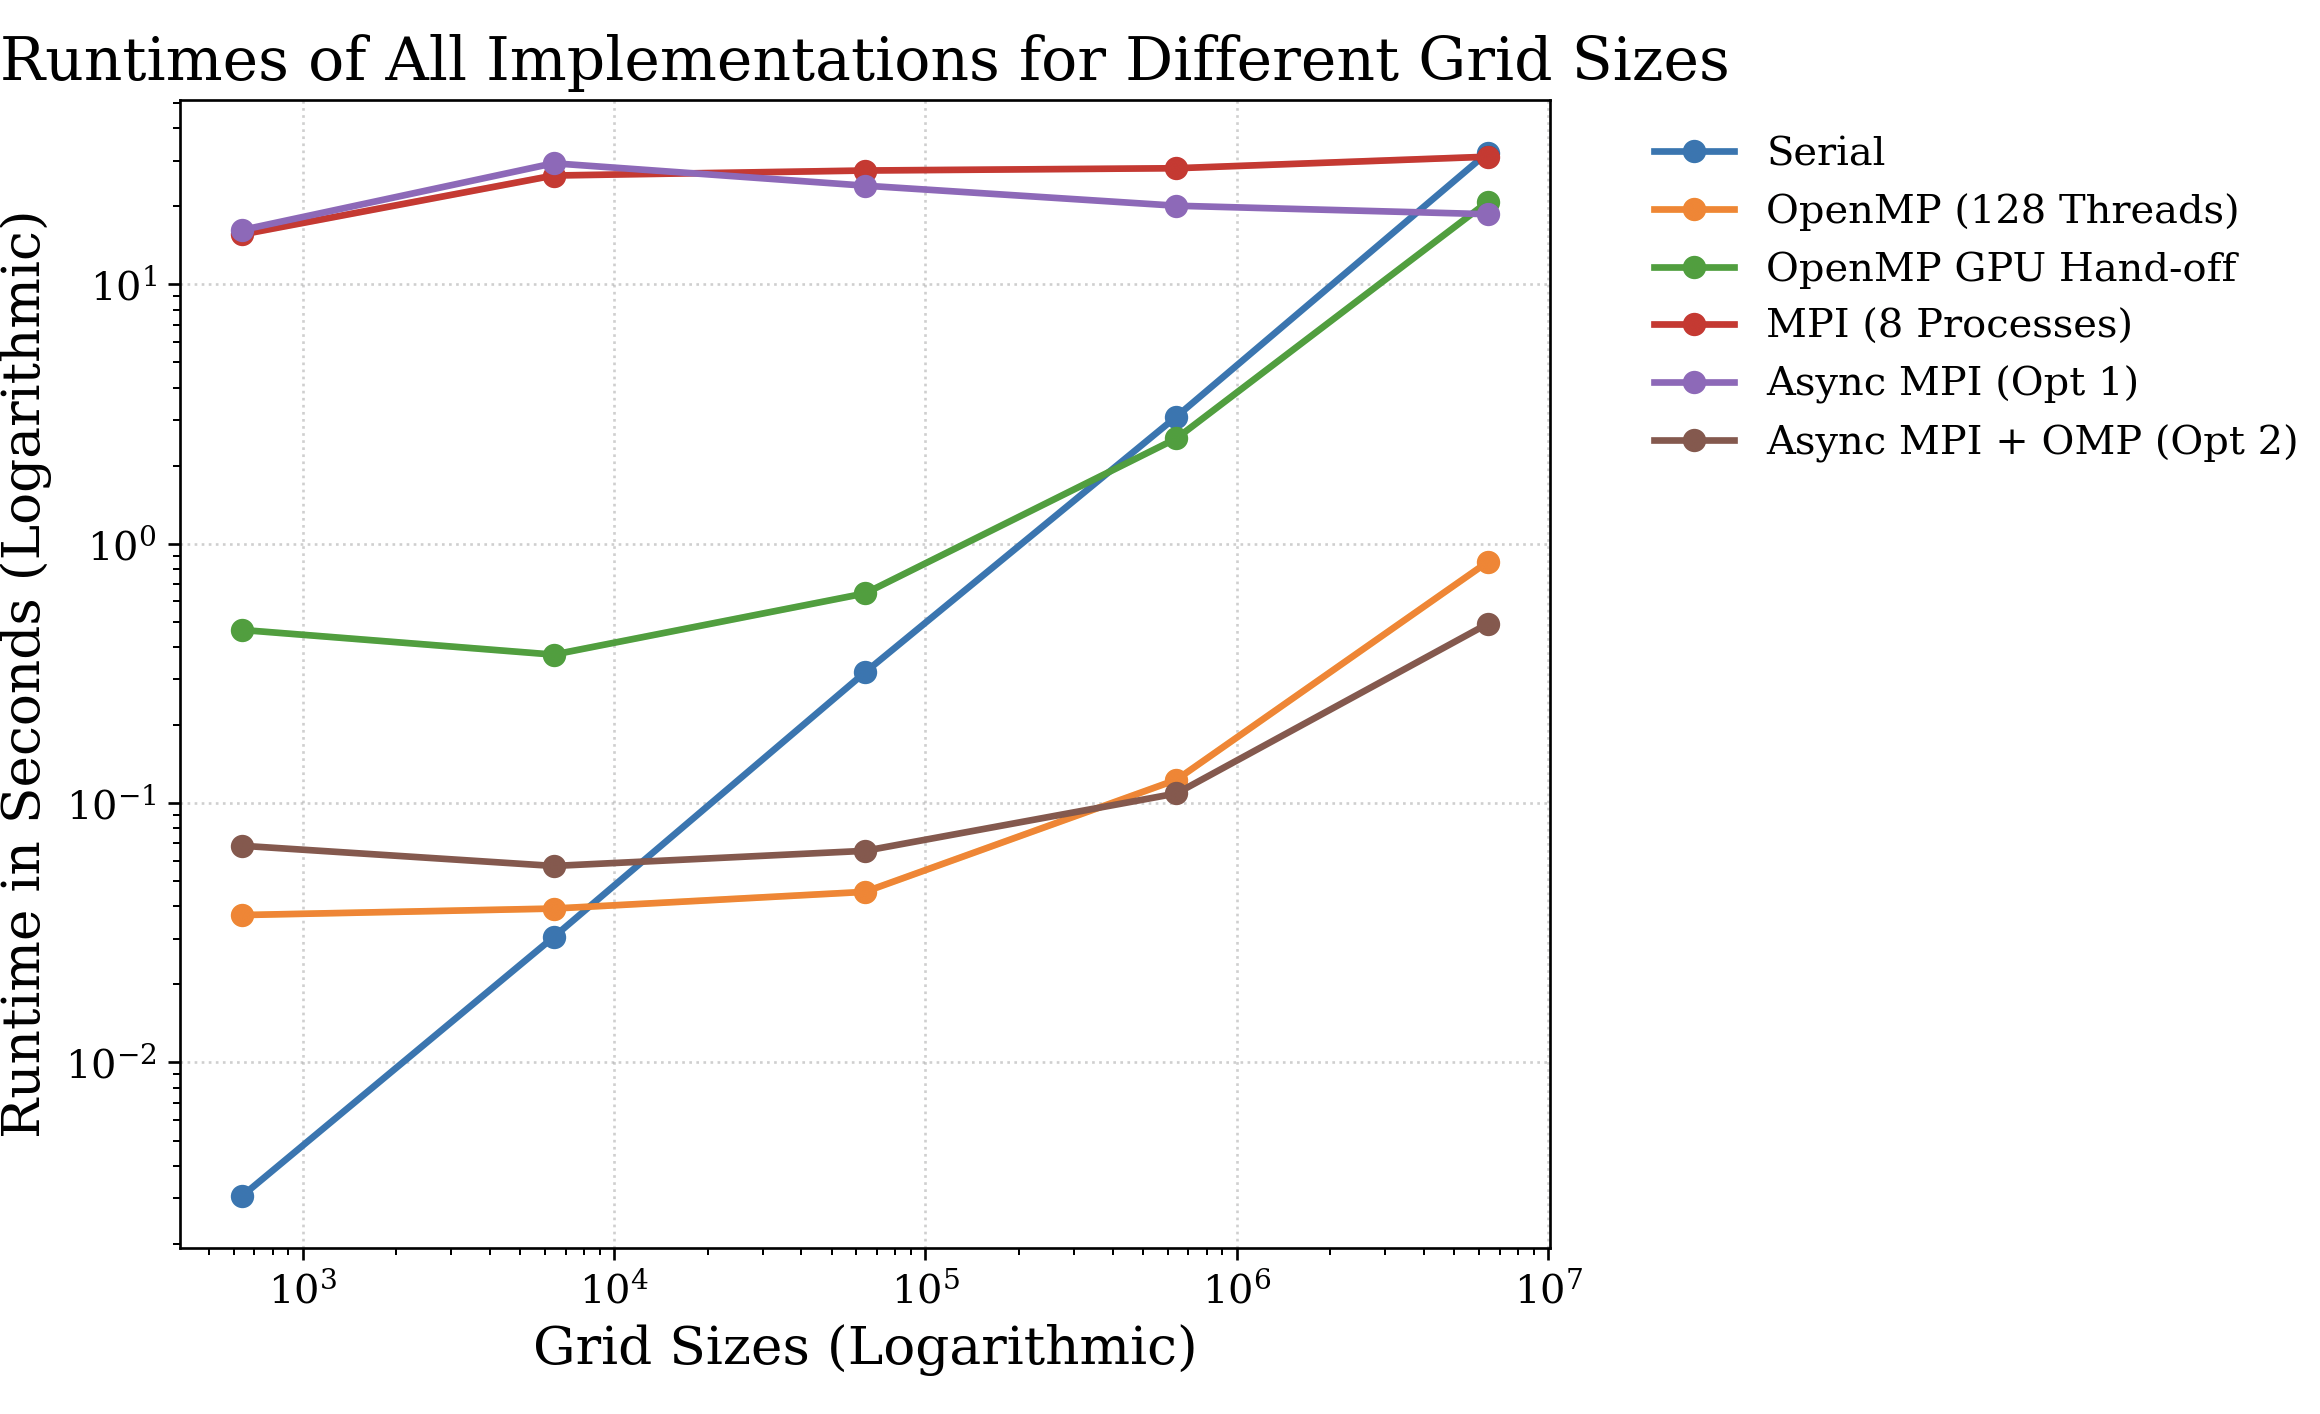
\includegraphics[width=0.9\textwidth]{../images/final_everything_plot.png}
  \caption{Concluding Results}
   \label{fig:conclusion}
\end{figure}

\todo{Do we really need to explain any of this? Keeping this here so we can remove later.}
One exception to this is the configuration chosen for the Base MPI implementation from Section \ref{sec:3_mpi}, where we chose 8 processes instead of 4 for this plot. As discussed earlier, we believe that the placement of the processes on a Dardel node by SLURM could play a non-trivial impact in determining the runtime of the blockimg MPI implementation (especially since there is no compute-overlap to \textit{hide} the cost of the communication). While 4 processes gave the lowest runtime in the strong-scaling test in Section \ref{sec:3_mpi}, it failed to give better runtimes than 8 processes when ran across different grid sizes in a separate run. As argued earlier, the runtimes for different 4 and 8 process counts in the Strong-Scaling test in \ref{sec:3_mpi} seemed to be within a margin of error from each other. Thus, we decided to go with 8 processes here, which gave lower runtimes on one of the runs (likely because of more favorable process-placements by Dardel on this run). 

From Figure \ref{fig:conclusion}, the serial implementation outperforms all parallel strategies for the smallest grid sizes, demonstrating that the overhead required to setup the different parallelization techniques overwhelms the amount of compute required to perform such small simulations. However, the serial implementation begins to be outshone by parallelization techniques very quickly.

The OpenMP implementations seem to perform the best out of all implementations, likely because of the sheer compute-acceleration offered by parallelizing the relatively simple and independend \verb|E| and \verb|H| updates in each simulation-iteration. Between these 2 approaches, the OpenMP only approach outperforms the MPI + OpenMP approach till a certain grid size. However, for the last 2 grid sizes, the Async MPI + OpenMP approach outperforms the raw OpenMP approach. This is likely because for bigger inputs, we begin to see the advantages of domain decomposition and better distribution of the input problem across different nodes and processes, reducing the load on a single node/process.

After these two implementations, we see that the GPU hand-off technique seems to perform reasonably well. The initial cost of moving the data to and from the GPU seems to overburden the runtime for smaller grid sizes, but as the grid size increases, we begin to see the advantage of GPU parallelization over the serial implementation. A way to improve the GPU parallelization even more in the future might be to explore involving multiple GPUs in the computation, which would require decomposing and distributing the problem manually across these GPUs. This might worsen runtimes for smaller grids, but might lead to better runtimes for much larger grids. 

Finally, the MPI-only implementations seem to perform very poorly for small-moderate grid sizes, likely because the overhead of the halo-exchange involved in the split-input domain does not offer any significant advantage over simpler implementations. This trend remains true for the Synchronous MPI implementation, which isn't able to take advantage of the communication-compute overlap. The Async-only MPI implementation, on the other hand, is able to overlap compute with communication for halo exchange and sees runtimes go down as the grid sizes increase (compared to serial and Sync MPI) as the compute is able to \textit{hide} the communication cost more effectively. \\

Thus, from this experiment, we believe that the best approach would be to use the \underline{serial} implementation for \underline{small input sizes}, then transition to the \underline{OpenMP only} approach for \underline{moderate input sizes}, and finally to switch the to the \underline{Async MPI + OpenMP} approach for \underline{large input sizes}. 

\section{Appendix}
\subsection{Std Dev, Min, Max Runtimes}
For brevity, we did not include the std dev, min, max of the runtimes obtained in the main report itself. The most important ones, however, be found in text-format in the repository, under the \verb|misc/stats_for_nerds| directory \href{https://github.com/paulmyr/DD2356-MethodsHPC/tree/master/5_project/misc/stats_for_nerds}{here}. Below we include some of the relevant files with these stats that might be of interest.
\begin{itemize}
\item \verb|serial_grid_vary.txt|: Serial runtimes for different grid sizes. Plotted in Figure \ref{fig:1_serial_runtime}.
\item \verb|omp_grid_vary.txt|: OpenMP Runtimes for different grid sizes (with 128 threads). Plotted in Figure \ref{fig:conclusion}.
\item \verb|omp_strong_scaling.txt|: OpenMP Runtimes for Strong Scaling test.
\item \verb|omp_weak_scaling.txt|: OpenMP Runtimes for Weak Scaling test.
\item \verb|gpu_grid_vary.txt|: GPU Runtimes for Different grid sizes.
\item \verb|mpi_strong_scaling.txt|: Runtimes for Strong-Scaling test of the base (sync) MPI implementation. Plotted in Figure \ref{fig:3_mpi_strong_scaling}
\item \verb|mpi_weak_scaling.txt|: Runtimes for Weak-Scaling test of the base (sync) MPI implementation. Plotted in Figure \ref{fig:3_mpi_weak_scaling}
\item \verb|sync_async_mpi_grid_vary.txt|: Runtimes for Base MPI (Sync) and Async (Opt 1) MPI implementation for different grid sizes using 8 processes. Plotted in Figure \ref{fig:4_opt_compare_8} and Figure \ref{fig:conclusion}.
\item \verb|async_mpi_process.txt|: Runtimes for Async MPI (Opt 1) implementation for same input size (6.4 million elements, 1k iteration), along with the Sync MPI runtimes in the same run. Plotted in Figure \ref{fig:4_opt1} and Figure \ref{fig:4_opt_all}.
\item \verb|async_omp_process.txt|: Runtimes for Async MPI + OpenMP (Opt 2) implementation for same input size. Plotted in Figure \ref{fig:4_opt_all}
\item \verb|async_omp_grid_vary.txt|: Runtimes for different grid sizes for Async MPI + OpenMP (Opt) implementation. Plotted in Figure \ref{fig:conclusion}
\end{itemize}

% content end
%###############################################################################

% \printbibliography

\end{document}
